\documentclass[a4paper]{article}
\usepackage[utf8x]{inputenc}
\usepackage{amsmath}
\usepackage{graphicx}
\usepackage[colorinlistoftodos]{todonotes}
\usepackage{textcomp}
\usepackage{multicol}
\usepackage{makeidx}
\usepackage{lstautogobble}
\usepackage{textgreek}
\usepackage[margin=1.25in]{geometry}
\usepackage[greek, english]{babel}
\usepackage{listings}
\usepackage{titlesec}
\usepackage{color}
\usepackage{fancyvrb}
\definecolor{gray}{gray}{0.5}

\lstset{basicstyle=\ttfamily,
  escapeinside=||,
  autogobble}
\newcommand{\tab}[1]{\hspace{.2\textwidth}\rlap{#1}}
\setcounter{secnumdepth}{4}
\titleformat{\paragraph}
{\normalfont\normalsize\bfseries}{\theparagraph}{1em}{}
\titlespacing*{\paragraph}
{0pt}{3.25ex plus 1ex minus .2ex}{1.5ex plus .2ex}

\title{\huge{Graphene}	\\	\LARGE{Project Report} \\ \large{COMS W4115 Programming Languages and Translators}} 

\author{Adith Tekur (at2904) \\ Pooja Prakash (pk2451) \\ Neha Rastogi (nr2477) \\ Sarah Panda (sp3206) \\ Sumiran Shah (srs2222) \\ \\
Team 8}

\date{\today}

\makeindex


\begin{document}
\begin{figure}
\centering
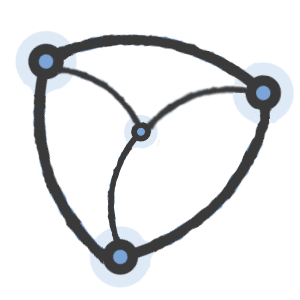
\includegraphics[width=0.3\textwidth]{logo.png}
\end{figure}
\pagenumbering{roman}

\newpage
\maketitle
\newpage
\tableofcontents
\maketitle
\pagebreak
\clearpage

\pagenumbering{arabic}
\setcounter{page}{1}

\section{White Paper}

\subsection{Motivation}
The motivation for our language is the massive commonplace use of graphs and graph based data mining algorithms in today's software world. At the same time, we see a large bubble of social network and social network-like applications which manage a large backend of data which can usually be represented using a graph structure. Most of today's languages do not provide out-of-the-box or easy to use features for graph initialization, operations and management. Our language aims to provide this interface to be able to support generic graph algorithms as well as specific social network applications based computations on graph-like data structures.
\newline

\subsection{Enter Graphene}
Graphene aims to fill the gap in existing programming languages by being one which is high level and easy to program and can be easily used by beginner programmers to analyze and manipulate graphs. Graphene is interpreted and easy to develop in and rapidly test. The compiler is lightweight and requires minimal setup and has a dependency only on python 2.7 to run.
\newline

\subsection{Target Audience}
The target audience for Graphene is twofold. First, beginner programmers who have little background in implementing and managing data structures in detail but wish to work on graphs. Second, organizations holding massive data in graph formats and who need to have dedicated computational services to model and mine data from graphs. Our language can be used to both, model new social networks as well as import data from existing dumps of social networks such as facebook, linkedin, twitter and compute on them.
\newline

\subsection{Buzzwords}
Graphene is \textbf{concise, dynamically typed, powerful, interactive, minimal development time, high level, interpreted}
\newline

\subsection{Salient Features}
Graphene supports powerful features of modern programming languages such as dynamic types, lambdas and multiple return parameters from functions. Graphene is interpreted and can be used to rapidly prototype, test and analyze data. It supports import and dumping of large graph files. Graphene comes with a powerful visualization library built with d3.js and jQuery which can be used to visualize clustering results or have user input data through a graphical user interface.

\subsection{Sample Program}
We present an example of a Graphene program which performs a common use case: a greedy method to find a minimal set of users of a graph which reach out to everyone in a graph. This can be used by advertisers or market researchers to identify a set of influential people.

\begin{verbatim}

/* Define a node type of 'person' with its attributes */
person has name,age;

/* Read input from file */
graph = input("person","data/0.edges");

/* User defined function to find the node with maximum outdegree in a graph.
   Input parameters : graph  : the graph to operate on.
   Output parameters: maxnode: the node with the maximum outdegree
*/
def (graph) => getNodeWithMaxDegree
{
    maxnode = graph.getNodes().first();
    maxdegree = graph.getAdjacent(graph.getNodes().first()).length();
    foreach(node in graph.getNodes())
    {
        curr = graph.getAdjacent(node).length();

        if(curr > maxdegr)
        {
            maxnode = node;
            maxdegree = curr;
        };
    };
} => (maxnode);

/* This is the core algorithm. It iteratively finds the node with maximum
   degree in the graph and eliminates it and its neighbours from the graph
   until all nodes are covered. It stores and returns the list of influential
   nodes used in each iteration.
   Input parameters : graph  : the graph to operate on
   Output parameters: Nodes  : the list of influential nodes found
*/
def (graph) => GlobalReach
{
    Nodes = [];
    while(graph.getNodes().length()!=0)
    {
        current = getNodeWithMaxDegree(graph);
        Nodes.append(current);
        foreach(node in graph.getAdjacent(current))
        {
            graph -= node;
        };
        graph -= current;
    };
} => (Nodes);

/* Call the function */
l = GlobalReach(graph);

/* Visualize the state of the program (all existing graphs) and highlight the
   influential nodes
*/
output().overlay(l);

\end{verbatim}

\begin{figure}[ht]
\centering
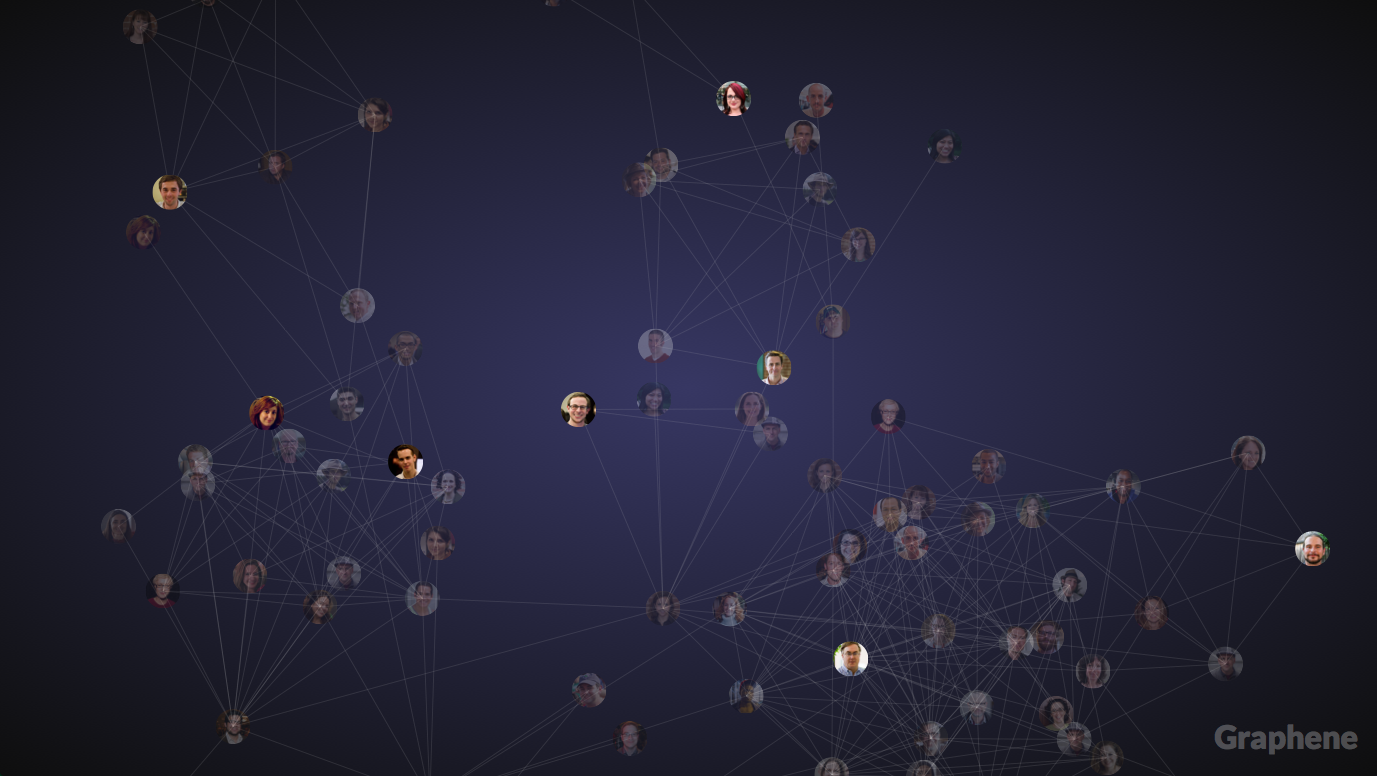
\includegraphics[width=1.0\textwidth]{screenshot.png}
\caption{Output of the above program.}
\end{figure}

\clearpage
\section{Language Tutorial}
\subsection{Introduction}

This tutorial is aimed to help a developer beginning in Graphene to ramp up on basic constructs and inbuilt functions. It is assumed that the developer has a beginner to moderate programming background and knowledge of graph data structures. In this section, we define the basic building blocks of the language, show how they interact and then provide sample code for a few common use cases.

\subsection{Language basics}

\subsubsection{Primitive data types}
\noindent Primitive data types which are specic to Graphene are:

\begin{enumerate}
\item Graph: A graph represents a collection of nodes interconnected by edges. A graph can be directed or undirected depending on whether or not the direction of edges have meaning. An edge connects two nodes of a graph. Similar to nodes, edges have a few implicit properties and more can be defined by key-value pairs in the associative property array.
\item Node: A node is an element amongst a set of similar elements of a graph. Each node has a few implicit language defined properties. User defined properties can be added as key-value pairs in an associative property array.
\end{enumerate}
\noindent Standard data types including String, int, float, double, char, boolean and lists of all types are also supported by our language.

\subsubsection{Declaring a graph}

\begin{figure}[ht]
\centering
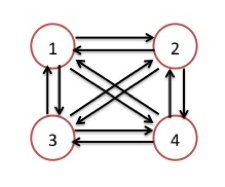
\includegraphics[width=0.3\textwidth]{mesh.png}
\caption{An example of a complete mesh graph.}
\end{figure}

\noindent Since a graph can be either directed or undirected, Graphene provides users with a type-specifier to indicate the same. $d$ and $u$ represent directed and undirected graphs respectively.
\begin{enumerate}
\item Inline from scratch
\begin{quote}
\begin{verbatim}
Graph g has d{ 1<-> 2, 1 <-> 3, 1 <-> 4, 2 <-> 3, 2 <-> 4, 3 <-> 4};
\end{verbatim}
\end{quote}
\noindent Here we list all edges of the graph. Two directional edges pointing in the opposite directions, or edges for undirected graphs are denoted by a $<->$ operator. A single directional edge can be specified by a $->$ operator. However, it may be easier to sometimes specify the edges absent from a graph which would otherwise be a full mesh network. For this, the user has can make use of method 2 as listed below.
\newline
\newline
The 'd' in initializer means that the graph is directed. If it were to be an undirected graph, the declaration should begin with a 'u' instead of a 'd'.
\newline
\newline
1, 2, 3 and 4 in the example represent ids of nodes. Node, a derived datatype in Graphene, is used to represent an entity which can be a part of (m)any graph(s). Nodes in graphene are universal and can be declared independent of graphs. A node can be associated with 0 or more graphs. However, an edge, unlike a node, is associated with a single graph. 
\newline
\item Inline from helper functions
\begin{quote}
\begin{verbatim}
g = mesh( nodecount , type );

e.g. g = mesh(4, d); /*This generates a graph as in Figure 1*/
g -= :1;
\end{verbatim}
\end{quote}
\noindent mesh(n) returns a full mesh graph containing n nodes. It automatically allocates unique IDs for the nodes ranging from 0 to (n-1). The code snippet creates a graph with 4 nodes and then removes node with id 1.

\item Import from dataset
\begin{quote}
\begin{verbatim}
g = input("person","data/0.edges");
\end{verbatim}
\end{quote}
\noindent To support the import of massive graphs, the input routine parses the file specified in the second parameter, treating nodes as the type specified in the first parameter. 'g' then is a reference to the parsed graph.

\item Graphical user input
\begin{quote}
\begin{verbatim}
g = input();
\end{verbatim}
\end{quote}
\noindent Calling the input routine without arguments invokes a browser to handle graphical user input for nodes and edges to a graph which is then assigned to 'g'. Through the graphical input, new nodes can be created by a left click on the empty background. \newline New edges can be created by clicking on the source node and dragging towards the destination node in the motion of "attaching".
User prompts ask for suitable attributes like weights for edges and names for nodes.
\end{enumerate}

\subsubsection{Declaring a node}
\noindent Nodes are inherited from a Node template. Therefore, to instantiate a node object, the user first declares a node type, specifying a list of keys that represent the attributes that objects of that node type possess. 
The following illustrates the example of creating a node type that represents a person, and subsequently, calls to the constructor returns a new object.
\begin{quote}
\begin{verbatim}
person has name,age;
person1 = person("Adam",21);
person2 = person("Bob",22);
\end{verbatim}
\end{quote}

\subsubsection{Properties of Nodes}
\noindent Each node has a unique node ID. A node can belong to multiple graphs. Hence, a node has a list of graph IDs to which it belongs to. A node in a graph may represent anything that can be modeled as a node in a graph. For example, in the domain of social network graphs, user accounts and pages can be represented as nodes. Hence, we allow for a user-dened list of properties through the $property$ parameter. For example, a user may specify "name" as a property of the node. This can be done as $property["name"]$. Assigning a value to this can be done using the = operator as $property["name"]$ = $<$value$>$.

\subsubsection{Properties of Edges}
\noindent Properties for an edge are defined in the context of graph declaration. Properties are a user defined list of key value pairs. Attribute of an edge can determine what the edge between two nodes signifies. It is this attribute that defines the relation between two nodes. If the two nodes connected by an edge represent user accounts, the edge may represent a relation of friendship between them or a relation of having similar interests. Such attribute gives the user the freedom to define node relations.

\subsection{Syntax}
\subsubsection{Comments}

Comments supported Graphene are the typical single-line and multi-line block.

\begin{quote}
\begin{verbatim}
/*
	This is a
	Graphene
	comment.
*/
\end{verbatim}
\end{quote}

\subsubsection{Operators}

We provide the basic arithmetic and logical operators. Other graph specific operators are as mentioned below.

\paragraph{Edge operators '$<->$', '$->$'}
    1$<->$2 represents a bidirectional edge between nodes 1 and 2. Depending on the graph, it may also represent an undirected edge. 1$->$2 represents an edge going from node 1 to node 2. 

\paragraph{Edge addition operator '+'}
\begin{quote}
\begin{verbatim}
	graphObj += "name":"Bob" -> "name":"John"; 
	graphObj += :1 <-> :2;
\end{verbatim}
\end{quote}

\noindent The edge addition operator accounts for both new nodes and new edges given in the expression. If the lookup node does not previously exist, edge addition fails.

\paragraph{Node removal operator}
\noindent The node removal operator is an equvalent complement to the node addition operator that is used to remove a node from a graph. An example is as follows.
\begin{quote}
\begin{verbatim}
		graphObj -= "name":"Alice";
\end{verbatim}
\end{quote}

\paragraph{Edge removal operator}
The edge removal operator can be used to remove an edge.
\begin{quote}
\begin{verbatim}

graphObj -= :2 -> :1; 
graphObj -= "name":"Alice"<->"name":"Bob";

\end{verbatim}
\end{quote}

\subsubsection{Control Flow}
The control flow of Graphene programs are very similar to any other programming language. The syntax of common control flow structures such as loops and conditionals are as follows.
\begin{quote}
\begin{verbatim}
if (expression)
{
/* matched first try! */
}
else if (some_other_expression)
{
/* that did not match, this did! */
}
else
{
/* nothing matched */
};

/* foreach loops */
foreach(n in graph.getNodes())
{
};
foreach(x in list)
{
};

/* for loops */
for (i = 0; i < 10; i++;)
{
};

/* while loops */
while (expression)
{
};
\end{verbatim}
\end{quote}

\subsection{Built In Functions}

\noindent Use of inbuilt library functions provide an intuitive sense of how to deal with the graph type.

\subsubsection{Shorthand notation}
\noindent "":"" is the supported way to handle stored key-value data.
\noindent By default, :id refers to value stored for key ID.

\begin{quote}
\begin{verbatim}
"key":"value"
:id  /*returns Node*/

nodeObj.["key"]; /*returns value for key*/
\end{verbatim}
\end{quote}

\subsubsection{General graph methods}
\begin{quote}
\begin{verbatim}
graphObj.getAdjacent(node); /*returns list*/
graphObj.getNonAdjacent("key":"value"); /*returns list*/

graphObj.hasNode("key":"value"); /*returns boolean*/
graphObj.hasNode(:id); /*default key is ID*/

graphObj.hasEdge("key":"value", "key":"value"); /*returns boolean*/
graphObj.hasEdge(:id, :id); /*default key is ID*/
\end{verbatim}
\end{quote}

\subsubsection{Node Handling:}

\begin{quote}
\begin{verbatim}
n = "key":"value"; /*returns Node*/
n = :id;

graphObj -= "key":"value"; /*returns boolean, true on success. */

\end{verbatim}
\end{quote}

\subsubsection{Node Degree calculations:}

\begin{quote}
\begin{verbatim}
graphObj.inDegree("key":"value"); /*returns number*/
graphObj.outDegree("key":"value"); /*returns number*/
graphObj.degree("key":"value"); /*returns number*/

\end{verbatim}
\end{quote}
$Note: Be\ cautious\ while\ calculating\ degrees\ for\ undirected\ graphs.\ degree\ != indegree + outdegree.\ This\ is\ because\ each\ edge\ counts\ only\ once.$

\subsubsection{Edge \& Node count:}

\begin{quote}
\begin{verbatim}
graphObj.getEdges().length();
graphObj.getNodes().length();
\end{verbatim}
\end{quote}


\subsection{User defined functions}
\begin{verbatim}
def (x,y) => doMath
{
    a = x+y;
    b = x-y;
    c = x*y;
    d = x/y;
} => (a,b,c,d);
\end{verbatim}
Each function definition is preceded by a 'def'. The input parameters are specified as an argument list in parenthesis and are always passed by reference. This is followed by the function name and the function body in curly braces. The body is followed by a return argument list in parenthesis similar to the input argument list.\\
In the above example, the function doMath takes two values x and y, and returns their sum, difference, product and quotient.

\subsubsection{Clustering based on user-specified lambda}
\begin{quote}
\begin{verbatim}
graphObj.cluster(lambda_expr);
\end{verbatim}

\end{quote}
\noindent $lambda\_expr$ is defined by the user and its signature is similar to that of a user defined function, with its syntax being of the form  $lambda(n1,n2):\{\}=>()$ which returns true if $n1$ and $n2$ are tested to belong to the same cluster. The nodes are updated with a clusterID attribute indicating the cluster they belong to.
\begin{quote}
\begin{verbatim}
e.g. graphObj.cluster(lambda(n1,n2): {} => (graphObj.hasEdge(n1,n2)));
\end{verbatim}
\end{quote}

\subsection{Sample Programs}

The following programs demonstrate different ways to use Graphene to manipulate and extract valuable information from graphs. We begin with a simple “Hello World” application that does the simplest operation of declaring a graph and adding a new edge to it.

\subsubsection{Hello World}

\begin{verbatim}
node has name;
node("A");node("B");node("C");node("D");
g has d {1<->2, 2->3, 3->2};
print("Hello World. The graph you defined has " + g.listNodes().count()
+ " Nodes ");
\end{verbatim}

\noindent This is a simple Hello World program. The first statement declares and initialises a directed graph named $g$ with nodes 1, 2, 3 and 4, and edges represented by the arrows between the nodes. The second statement prints “Hello World..” along with the number of nodes and edges in the graph found using the built-in functions for a Graph object.
\newline

\subsubsection{Scenario: Create a network, identify all the closely-knit groups and find
who is the go-to person in each.}
\begin{quote}
\begin{verbatim}
def (G) => findMostInfluential
{
    Subgraphs = g.cluster(lambda (n1,n2) => {} => (g.hasEdge(n1,n2)));
    maxdegree = 0;
    degree = 0;
    Maxinfluential = 0;
    foreach(graph in Subgraphs)
    {
        maxdegree=0;
        influential = graph.getNodes().first();
        foreach(user in graph.getNodes())
        {
            degree = graph.inDegree(user);
            if(maxdegree < degree)
            {
                maxdegree = degree;
                influential = user;
            };
        };
        Maxinfluential.add(influential);
    }
} => (Maxinfluential);

Graph g has d{ 1->2,3->5,2->5,3->4 };
gotoperson = findMostInfluential(g);
print("Found "+ gotoperson.length() + "Closely-Knit groups");
output(g).overlay(gotoperson);
\end{verbatim}
\end{quote}

\subsection{Executing a Graphene program}

Graphene is interpreted and is very simple to execute. Graphene source files conventionally end in a ".ene" extension. If a source file with no extension is specified, the compiler will still try to interpret it as a plain-text file containing graphene source code.

The Graphene interpreter can be summoned by "graphene" followed by the source file name.

eg: Consider a source file called "graph.ene". It can be run by:

\begin{verbatim}
$ ./graphene -f graph.ene
Hello, World!
$
\end{verbatim}

Graphene also features a REPL to execute statements line by line incrementally. The REPL can be initialized by simply calling the graphene script without any parameters as such:

\begin{verbatim}
$./graphene
graphene> print("Hello, World!");
Hello, world!
graphene> 
\end{verbatim}

\newpage
\section{Language Reference Manual}
\subsection{Introduction}

	In this manual, we describe the various features of Graphene that can be used in defining and manipulating graphs. We present an overview of the lexical conventions, syntax of the language and the grammar representing Graphene.

\subsection{Lexical Conventions}

Like for every language, Graphene is composed of lexemes following patterns represented by tokens. Apart from whitespaces (that represent spaces, tabs and newlines) and comments, our language has the tokens - identifiers, keywords, constants, operators and separators.


\subsubsection{Comments}

Graphene provides support for multi-line comments. Comments on the other hand bengin with "/*" and and with "*/". An example is as follows.

\begin{quote}
\begin{verbatim}


/* This is a...
...multi-line comment */ 

\end{verbatim}
\end{quote}
Note that one multi-line comment cannot be nested within another multi-line comment.

\subsubsection{Identifiers}

\noindent An identifier represents a unique entity within a program. Graphene follows the naming convention specified below.

\begin{enumerate}
\item An identifier can be any sequence of alphabets, digits or underscores.
\end{enumerate}

\noindent Graphene is case-sensitive.

\subsubsection{Keywords}
The following keywords convey special meaning to Graphene and hence should not be used elsewhere.

\begin{multicols}{2}
\begin{quote}
\begin{verbatim}
def
if
else
return
while
for
foreach
in
has
on
Graph
Edge
d{
u{
->
<->
lambda
True
False
\end{verbatim}
\end{quote}
\end{multicols}

\subsubsection{Reserved}
The following characters are reserved for use in the grammar.

\begin{multicols}{5}
\begin{quote}
\begin{verbatim}
+ 	
- 	
*
/	
%
( 	
) 	
{ 	
} 	
[	
]
=
==	
!=	
<	
>	
>=	
<=
&&	
||	
!
.	
,	
;	
->
<->
'
"
+=
-=
:
=>
\end{verbatim}
\end{quote}
\end{multicols}

\subsection{Types}

\subsubsection{Basic Types}
Graphene handles type dynamically. 
Basic data-types recognized and handled approriately are:

\begin{quote}
\begin{enumerate}
\item int - This is used to define integer numbers. Data of the form $[0-9]*$ will be handled as type $int$.
\item float - This is used to define floating-point numbers. $[0-9]+.[0-9]+$ translates to type $float$.
\item boolean - Values 'True' or 'False' will define $boolean$ type.
\item string - This is used to represent strings (sequence of characters enclosed within $""$ or $'$ $'$).
There is no char type. Instead, it is handled as a string made of 1 character. This eliminates the need to handle $'$ and $"$ differently.
\end{enumerate}
\end{quote}
All the basic data-types - int, float, char and boolean can also be represented in Graphene as a string (sequence of characters enclosed within ""). 
\newline
\newline
The type of the variable is determined dynamically on the basis of the the characters enclosed and is handled accordingly. 

The following is one such example.

\begin{multicols}{2}
\begin{quote}
\begin{verbatim}
integerVar = 70;		
floatVar = 50.5;		
boolVar = True;		
stringVar = "graphene";
//integerVar is handled as an integer
//floatVar is handled as a floating point
//boolVar is handled as boolean.
//stringVar is handled as a string
\end{verbatim}
\end{quote}
\end{multicols}

\subsubsection{Derived Types}
The following are the derived data-types supported by Graphene.
\begin{quote}
\begin{enumerate}
\item Graph - This is used used to define graphs.
\item Node - This is used to define a node in terms of user-defined properties representing the node. Graphene assigns a unique id to every node that is created. In other words, the id$s$ of the nodes are globally unique. 
\item List - Graphene supports arrays to represent multiple entities of the same type. An element within an list can be accessed using its index (Ex. l[0] retrieves the first element of the list l).
\end{enumerate}
\end{quote}

\subsubsection{Escape Sequences}
The following escape sequences are supported by Graphene.

\begin{multicols}{2}
\begin{quote}
\begin{verbatim}
\n	
\t	
\\	
\'	
\"	
newline
tab
backslash
single quote
double quote
\end{verbatim}
\end{quote}
\end{multicols}

\subsubsection{Boolean Constants}
The boolean constants supported by Graphene are True and False.

\subsection{Scope}
\subsubsection{Block Scope}
Variables declared in a block are valid only for that block. A block can be a part of the function definition.

\subsubsection{Function Scope}
Variables declared in a function are valid only within that function. Once the function returns, the variables declared within the function are no longer visible.

\subsubsection{Global Scope}
Variables declared outside the functions are valid for all the functions in that program.

\subsubsection{Lexical Scope}
A variable's scope is based only on its position within the textual corpus of the code. Variable names in the same scope must be unique.

\subsubsection{Linkage Scope}
External library function or constants can be accessed through their identifiers and are shared by the entire program.

\subsection{Grammar}
\begin{quote}
\begin{lstlisting}
  S :  
  	program
  
  program :  
  	declarationlist
    
  declarationlist :  
  	declaration declarationlist
  	declaration
  
  declaration :  
  	funcdec
  	vardec
    
  vardec :  
  	node-dec ;
  	graph-dec ;
  
  node-dec :  
  	ID HAS keylist
  
  keylist :  
  	idOrAlphanum
  	idOrAlphanum COMMA keylist
  
  graph-dec :  
  	GRAPH ID HAS GRAPHTYPE edgelist CURLEND
  	GRAPH ID HAS GRAPHTYPE edgelist CURLEND ON idOrAlphanum
  
  edgelist :  
  	idOrAlphanum CONNECTOR idOrAlphanum
  	idOrAlphanum CONNECTOR idOrAlphanum COMMA edgelist
  	idOrAlphanum CONNECTOR idOrAlphanum LPAREN arglist RPAREN
  	idOrAlphanum CONNECTOR idOrAlphanum LPAREN arglist RPAREN COMMA 
    	edgelist
  
  declaration :  
  	statement
  
  statement :  
  	compoundstatement
  
  compoundstatement :
  	CURLBEGIN statementlist CURLEND
    CURLBEGIN CURLEND
  
  funccompoundstatement :  
  	CURLBEGIN statementlist CURLEND
  	CURLBEGIN CURLEND
  
  funcdec :
  	func ;
  
  func :  
  	DEF parameters IMPLY ID funccompoundstatement IMPLY returnarguments
  
  lamda :  
  	LAMDA parameters COLON funccompoundstatement IMPLY returnarguments
  
  assignmentexpression :  
  	ID = lamda
  
  parameters :
  	LPAREN RPAREN
  	LPAREN varargslist RPAREN
  
  varargslist :
  	varargslist COMMA ID
  	ID
    
  returnarguments :  
  	LPAREN RPAREN
    LPAREN returnset RPAREN
    
  returnset :  
  	expression
  	expression COMMA returnset
    
  statementlist :  
  	statement
  	statement statementlist
  
  statement :  
  	expressionstatement
  	iterationstatement ;
  	selectionstatement ;
    
  edgeaddition :  
  	ID ADD_STORE idOrAlphanum CONNECTOR idOrAlphanum
  
  
  noderemoval :
  	ID REMOVE_STORE nodeLookup
   
  nodeLookup :
  	idOrAlphanum COLON idOrAlphanum
 		COLON idOrAlphanum
  
  iterationstatement :
  	WHILE LPAREN expression RPAREN statement
  	FOR LPAREN statement expression ; statement RPAREN CURLBEGIN 
    	statement CURLEND
  	FOREACH LPAREN ID IN ID RPAREN CURLBEGIN statementlist CURLEND
  	FOREACH LPAREN ID IN expression RPAREN CURLBEGIN statementlist
    	CURLEND
  
  selectionstatement :  
  	IF LPAREN expression RPAREN compoundstatement
  	IF LPAREN expression RPAREN compoundstatement ELSE 
    	compoundstatement
    
  expressionstatement :  
  	;
  	completeexpression ;
    
  completeexpression :  
  	callchain
  	assignmentexpression
  	dgeaddition
  	noderemoval
    edgehasproperty
  
  edgehasproperty :
  	ID DOT SQRBEGIN STRING = idOrAlphanum SQREND
  
  expression :  
  	ID DOT SQRBEGIN STRING SQREND
  
  assignmentexpression :  
  	ID = expression
  	arglist = expression
  	ID = nodeLookup
  	ID = SQRBEGIN values SQREND
  	ID = SQRBEGIN SQREND
 	ID = ID SQRBEGIN SQREND
  	ID SQRBEGIN idOrAlphanum SQREND = idOrAlphanum
  	ID SQRBEGIN idOrAlphanum SQREND = SQRBEGIN values SQREND
    
  values :  
  	valuelist
    
  valuelist :  
  	idOrAlphanum COMMA valuelist
  	idOrAlphanum
 
 expression :
  	expression + expression
  	expression - expression
  	expression % expression
  	expression * expression
  	expression / expression
  
  expression :
  	expression LS expression
  	expression GR expression
  	expression GRTEQ expression
  	expression LESSEQ expression
  
  expression :
  	expression LOGAND expression
  	expression LOGOR expression
  	expression EQUAL expression
  	expression NEQUAL expression
  
  expression :
  	LPAREN expression RPAREN
  
  expression :
  	idOrAlphanum
  
  expression :
  	ID SQRBEGIN idOrAlphanum SQREND
  
  expression :
  	callchain
  
  callchain :
  	call
  	call DOT callchain
  
  call :
    ID LPAREN callarglist RPAREN
    ID DOT ID LPAREN callarglist RPAREN
    ID DOT ID LPAREN RPAREN
    ID LPAREN RPAREN
  
  callarglist :
    expression COMMA callarglist
    expression
  
  arglist :
    idOrAlphanum COMMA arglist
    idOrAlphanum
  
  idOrAlphanum :  
    NUMBER
    TRUE
    FALSE
    STRING
    ID

\end{lstlisting}
\end{quote}

\subsection{Grammar Explanation}
\subsubsection{Lambda Functions}
\begin{verbatim}
    lamda :  
  		LAMDA parameters COLON funccompoundstatement IMPLY returnarguments
\end{verbatim}

\indent A lambda function, defined by beginning with the keyword "lambda", can be used by a user to specify the logic on the basis of which functions utilizing lambdas can perform manipulations. For example, clustering functions will accept a lambda function as their first argument that specifies the heuristic for grouping of nodes into clusters. The keyword lambda identifies such a function. Like regular functions, lambda functions takes in zero or more comma separated list of arguments. A comma separated list of arguments can be returned.
Built-in functions will specify the signature of the lambda they except. A mismatch will result in a compile error.

\subsubsection{User-defined Functions}
\begin{verbatim}
    func :  
  		DEF parameters IMPLY ID funccompoundstatement IMPLY returnarguments
\end{verbatim}

\indent User-defined functions, beginning with the keyword "def", are structurally similar to lamba functions except that the first argument may be a lambda function. Note that in the presence of a lambda function, it has to always be the first argument that is passed. Like in lambda functions, Graphene supports multiple return values.

\indent A user-defined function can accept a lambda as an optional first argument. A lambda however, cannot accept another lambda as an argument.

\subsubsection{Function Calls}
\begin{verbatim}
    call :
      ID LPAREN callarglist RPAREN
      ID DOT ID LPAREN callarglist RPAREN
      ID DOT ID LPAREN RPAREN
      ID LPAREN RPAREN
\end{verbatim}

\indent A function call consists of the name of the function followed by its arguments. The return value of this function can in turn call another function, providing for function chaining.

\subsubsection{Handling Multiple Return Arguments}
\begin{verbatim}
    assignmentexpression :
  		arglist = expression
\end{verbatim}

\indent Graphene provides out-of-the-box support for multiple return arguments. A list of variables can then form the LHS for a function call that returns multiple values. In the event of mismatch of number of arguments, an error is generated.

\subsubsection{Nodes}
\paragraph{Declaration}
\begin{verbatim}
   node-dec :  
  	ID HAS keylist
\end{verbatim}

\indent Graphene allows users to define properties that represent a node. These properties are typically key-value pairs. The user can define a universal set of keys for a particular node type. The "has" keyword implies that the node should contain values for at least the specified set of keys.

\paragraph{Initialization}
\begin{verbatim}
    assignmentexpression :  
  		ID = expression
    
\end{verbatim}

The above production rule is used to initialize nodes by assigning values to the keys of their corresponding types. The \$id is the unique id of the node. kv-list represents the set of values to be assigned to the keys defined. The expression in this scenario is a call to the Nodetype, which calls the constructor with the actual values of members of the node object. \newline

An example of the declaration and initialization of a node is as follows.

\begin{multicols}{2}
\begin{quote}
\begin{verbatim}
Person has name, school;
Person1 = Person("John", "CU");


//Declaring a node-type Person

//Assigning values to keys of 
//Person for node Person1
\end{verbatim}
\end{quote}
\end{multicols}

\subsubsection{Graphs}
\paragraph{Declaration \& Initialization}
\begin{verbatim}
  graph-dec :  
  	GRAPH ID HAS GRAPHTYPE edgelist CURLEND
  	GRAPH ID HAS GRAPHTYPE edgelist CURLEND ON idOrAlphanum
\end{verbatim}

\indent A variable of graph data type can be declared using the edge list and a keyword which represents whether the graph is directed or not. 
graph-type is "u" for undirected graphs and "d" for directed graphs. 
Edge list contains the list of all edges along with the connector which represents the direction of the edges. Connector $"->"$ refers to a directed edge in a single direction and $"<->"$ refers to directed edges in both directions. The latter also represents the edge in an undirected graph.
 

\newpage
\section{Project Plan}
With the knowledge that planning and organization are the key aspects of this project, we started the discussions on the language ideas in last week of January. After a series of meetings and brainstorming sessions, we came up with a number of unique ideas pertaining to  a wide range of application domains. After close consideration of the feasibility of each idea, interest of team members and discussion with Professor.Aho, we decided on the idea of developing Graphene. To track all the ideas and the meeting notes, we used Flowdock and to shortlist ideas as per interest, we used doodle. We also created a Github repository at the same time for version control.

\subsection{Planning}
Throughout the project, we followed an iterative planning process, where we initially set the main goals and milestone deadlines and then iteratively created short-term goals as we moved further in the project. After finalizing the language, we decided to meet twice a week to figure out the language specifications and other project milestones. One of the main tasks as was mentioned by the professor was to decide on the roles of every team member. After finalizing the roles and delegating the responsibilities to each member, we started with the Language Whitepaper, which was due on Feb 26th. We used Google docs to collaborate on it and then used writelatex.com to convert it into latex format. 

\subsection{Specifications}
Once we gained an understanding about the whole process, we met with the TA’s to discuss the scope of the implementation and to verify if we were moving in the right direction. We submitted the Language tutorial and LRM on March 26th and then we started the implementation of the language. We decided to first develop the basic structures needed for the language and then proceed further. So we started with first implementing the Hello World program.

\subsection{Development}
We decided to develop the lexer and parser first for the basic language constructs so that we can implement the Hello World program. Once that was done, we moved on to develop the classes for Abstract Syntax Tree and for traversing the tree to produce the output. As we maintained a Github repository, so that enabled all the team members to work on their respective parts and commit the code in their own branch. We kept on updating the main branch from these individual branches on a timely basis. This technique helped us to prevent any major mishaps with the code and also easy to track if something goes wrong.

\subsection{Testing}
In order to verify that the compiler code is working correctly after every incremental change, we developed a testing framework using a Python’s module viz. Pexpect. We added test cases to the framework as and when new features were implemented. This approach also helped us learn if the new changes broke any already existing feature and hence fix the problem. The detailed description of our test plan and framework is covered in Chapter 8 of the report.

\subsection{Responsibilities}
On a high level, responsibilities were divided across the team members as in the table below, however, this division wasnt strict in action, as multiple team members contributed to multiple parts of the language, depending on the stage of the project, as well as expertise, interest and availability of the indvidual members.\\
\begin{figure}[h]
\centering
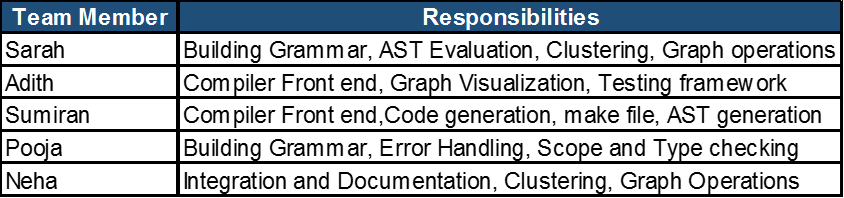
\includegraphics[width=1.0\textwidth]{graphene.png}
\end{figure}


\subsection{Implementation Style Sheet}
We used the following rules when writing our code to ensure maximum readability -\\
\hspace{.4cm}Each line of the code should remain under 100 characters.\\
\hspace{.4cm}Write utility functions for commonly reused code.\\
\hspace{.4cm}Use self documenting variable names.\\
\hspace{.4cm}Use underscore separated function names.\\


\subsection{Timeline}

\begin{figure}[h]
\centering
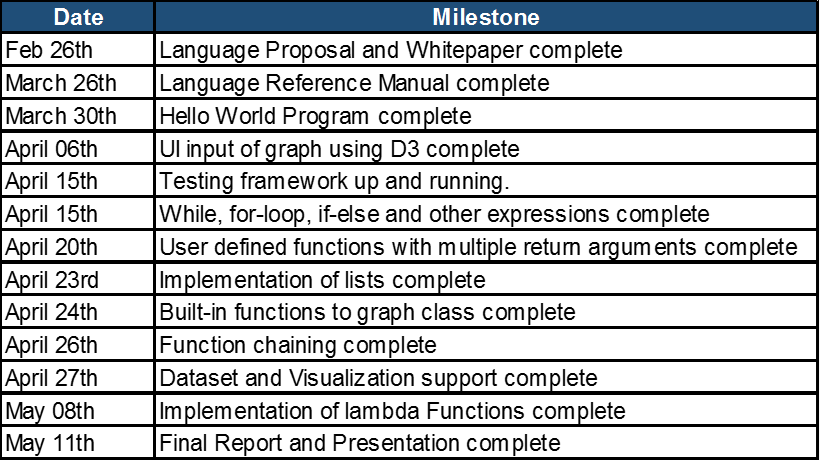
\includegraphics[width=1.0\textwidth]{timeline-1.png}
\end{figure}

\newpage
\section{Language Evolution}
The main feedback we received on our Language Reference Manual during the early stages of development of Graphene was that our grammar was huge which would make the implementation of the kernel difficult in the given time-frame. We hence worked incrementally towards implementing the grammar. We started off with the basic constructs constituting the kernel and then went on to implementing sophisticated features. This approach proved to be helpful in that we had a solid infrastructure right in the beginning on top of which the rest of the language framework was built.


\subsection{Compiler Tools}

Considering the programming background of all the team-members of Graphene, we came up with a unanimous decision of having Python as the target language for our compiler. We used Python’s Python Lex-Yacc (PLY) for implementing the lexer and the parser for our compiler. Apart from the ease of use, Python provided us with an added advantage of being extensively documented making debugging and bug-fixing relatively simple.\\

\noindent For developing the testing framework, we used Pexpect, another Python module. Quoting from "pexpect.sourceforge.net", Pexpect is a module for spawning child applications and controlling them automatically.\\

\noindent The code for building and traversing through the Abstract Syntax Tree (AST) representing the syntatic structure of Graphene was written in-house.\\

\subsection{Libraries}
We use Data Driven Documents (D3) for developing the UI supporting the input and output of graphs. As stated by D3, it is a Javascript library for manipulating  documents based on data. It combines powerful visualization components using HTML, SVG and CSS.\\

\noindent The interpreter accepts inputs made through this UI and converts it into the internal representation of Graphene for the purpose of further processing. Conversion back to the visual representation of the graph is done for displaying it to the user through the UI.\\

\subsection{Consistency}
After receiving the feedback on the size of our grammar and further realizing that we would not be able to implement the whole, we updated the LRM with the new grammar. We removed several constructs which we deemed insignificant at later stage. One such example is that we removed the grammar related to edges and its operations.


\newpage
\section{Translator Architecture}
\begin{figure}[h]
\centering
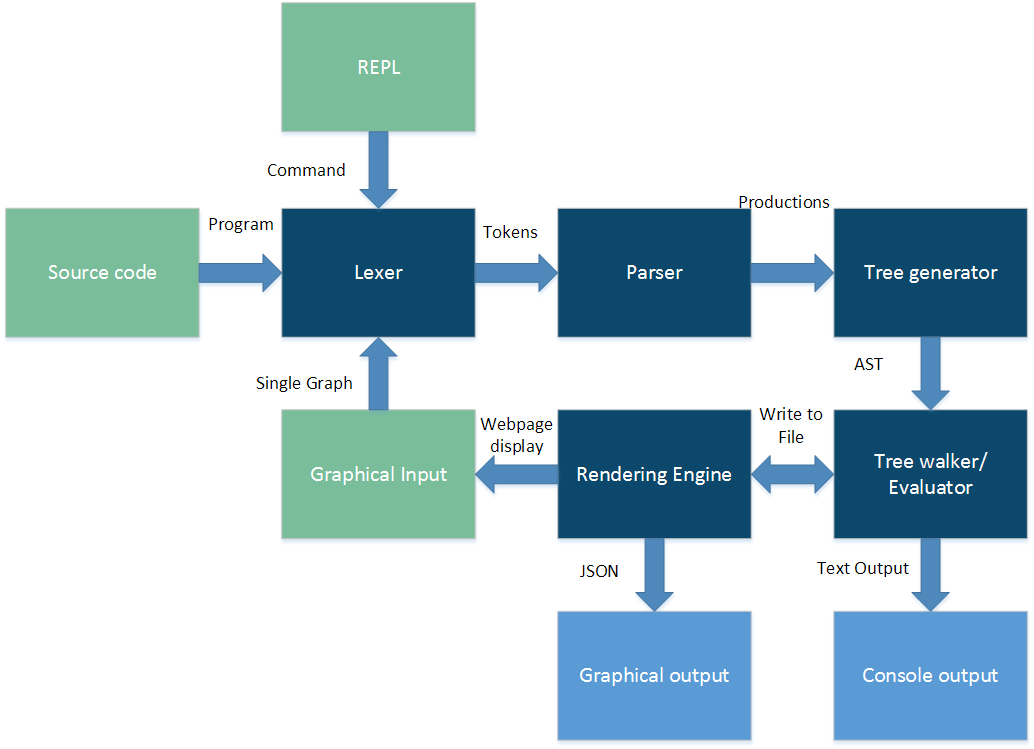
\includegraphics[width=1.0\textwidth]{FlowDiagram.png}
\end{figure}

\subsection{Pre-Processor (Graphical Input)}

In order to show the usefulness of Graphene specific to social media networks, retrieving a fair representation of such data was necessary. So, we downloaded facebook data from the Stanford Large Network Dataset Collection(SNAP). One major problem that we faced was that the entire dataset was anonymized, so there were no attribute values correspoding to the nodes. Showing the functionalities that Graphene has to offer with such anonimized data was not possible. As a solution to this, we assigned random attribute values to the nodes in this social network graph. This random data was obtained from a free API for generating random user data - randomeuser.me. 
As part of preprocessing this integrated data-set is converted to Graphene's internal representation. The user also has the option to draw a graph using the Rendering Engine. The graph so obtained acts as an input to the lexer.

\subsection{Lexer}
The lexer tokenizes the input into Graphene readable units. This process includes discarding whitespaces and comments. The lexer then outputs recognized tokens which in turn act as inputs to the parser.

\subsection{Parser}
The parser communicates with the lexer and receives tokens from the lexer one by one and tries to match them with the grammar specifications. As the parser evaluates these tokens, it also adds them to the Abstract Syntax Tree (AST). In other words, we add the lexemes identified by the lexer as nodes of the AST. The final AST will thus include the whole tree of the parsed program. We have implemented a separate library file for AST handling, the major chuck of whose code is in the class - ASTNode.

\subsection{Rendering Engine}
\noindent Data flow from the interpreted program and the webpage is in the form of JSON. The current state to be represented is written to a pre-determined file and the template webpage is launched, served by an ephemeral server that responds to requests for a short period of time before killing itself. The webpage then makes an AJAX call (asynchronous GET request), loads the state and processes the display formation. \\

\noindent In the case of loading anonymized facebook data, at the input stage itself, as shown in the Whitepaper section, nodes without attributes are provided with randomly generated user information to help visualize the data.


\subsection{Tree Generator}
As the input program is parsed, relevant nodes are created in the AST and/or mapped as children to newly created nodes, according to the semantic action defined against the respective production rule. Each created node is assigned a type upon creation. The ASTNode.type determines the action to be performed on the node and the return value. This structure is useful when the tree is evaluated using the following module.

\subsection{Tree Evaluator}
Since Graphene is an interpreted language, the final step is to walk the AST and produce the output. The AST prepared from the previous step is now mapped to the corresponding python code and that code is executed to give the output of the program. The output includes text output on the console or the graphical output using the rendering engine.


\newpage
\section{Development \& Runtime Environment}
The compiler was developed in mainly two environments - Windows 7 and Mac OS. The team members used sublime or notepad++ for editing the code and command line or terminal for testing. As already mentioned before, we used Github as the source repository to track the changes. Since Python 2.7.6 was the most stable version and most widely used version, we settled for that.\\

\noindent In addition to these, we also used Google Hangouts for remote meetings allowing face to face interaction. We also used messaging services like WhatsApp and the traditional e-mails to effectively communicate. We also used FlowDock, which is a team collaboration application, to keep everyone in loop.\\

\noindent During development, we used a bash script which handles command line arguments to call the graphene compiler in debugging mode or to execute regression tests. The makefile makes a simple call to this bash script.\\

Bash script to launch graphene:

\begin{verbatim}
#!/bin/bash
usage() {
  echo "Usage: graphene [test [-t <number>]|[-i]] | [-f <file_path>] | -h "
}
if (($# == 0)); then
  python graphene.py
else
  if [ $1 = "test" ]; then
    if (($# == 1)); then
      python test/main.py
      exit 1
    else
      if (($2 == "-i" )); then
        # "Scotty! I need.. more.. isolated tests!"
        python test/main.py -i
        exit 1
      elif (( $2 == "-t" )); then
        if (($# != 3)); then
          usage
          exit 1
        fi
        # "Run this, sesame!"
        python test/main.py -t $3
        exit 1
      else
        usage
        exit 1
      fi
    fi
  fi
  args=" "
  while getopts ":f:t:idh" opt; do
    case $opt in
      f)
        args+=" -f $OPTARG"
        ;;
      
      d)
        # "I don't always know what's going on.. But when I do, I don't!"
        args+=" -d"
        ;;
      h)
        echo "Help is at hand." >&2
        echo "OPTIONS"
        echo -e -n "\t-f"
        echo -e "\tFile to read source from"
        echo -e "\t\tUsage: graphene -f <path>"
        echo -e -n "\n\t-t"
        echo -e "\tRun test Number <number>"
        echo -e "\t\tUsage: graphene test -t <test_name>"
        echo -e -n "\n\t-i"
        echo -e "\tRun tests in isolated mode. One test does not affect another."
        echo -e "\t\tUsage: graphene test -i"
        break
        ;;
      \?)
        echo "Invalid option: -$OPTARG" >&2
        exit 1
        ;;
      :)
        echo "Option -$OPTARG requires an argument." >&2
        echo "Usage: graphene [test | -t <number> | -i | -f <file_path>] "
        exit 1
        ;;
    esac
  done
  python graphene.py $args
fi
\end{verbatim}




\newpage
\section{Test Plan}
\subsection{Tools}
In order to ensure that newly added code does not break the already existing code, regression testing was required. In order to do so, we had a testing framework in place early on to which test cases were added to test every change and addition made. As mentioned earlier, the testing framework makes use of the Python module called Pexpect for writing the test script.

\subsection{Testing Framework}
Our testing framework is defined in the file tests/main.py. This file defines a series of tests that help verify the correctness of every section of the code. Each test case includes mainly two aspects - test code and expected output. The verification of correctness is then done by comparing the output generated for each case with the expected output for the same. We started off with a few test cases and added more cases incrementally to test newly added constructs. Testing individual constructs against testing the entire code proved to be helpful in easily narrowing down on sections that caused errors.\\

\noindent The code implementing the testing suite is as follows.

\begin{verbatim}
#!/usr/bin/env python
# -*- coding: UTF-8 -*-

from __future__ import absolute_import
from __future__ import print_function
from __future__ import unicode_literals

from itertools import cycle
import os.path
from collections import OrderedDict
import logging

import sys
import pexpect
import time
import json

TEST_LOG = "test/test.log"
MINOR = "MINOR"
CRITICAL = "CRITICAL"
PANIC = "PANIC"
PASS = 1
FAIL = 0
log = None

tests = OrderedDict()
tests = {
//Add test cases here
}

failed_tests = []

PROMPT = "graphene>"
print("\n\n")

c = pexpect.spawn('/usr/bin/python graphene.py')
c.expect(PROMPT)
ran = 0
failed = 0
isolated = False
test_name = -1

if len(sys.argv) >1:
    if sys.argv[1] == "-i":
        isolated = True
    elif sys.argv[1] == "-t":
        test_name = sys.argv[2]

for name, test in tests.iteritems():
    if test_name != -1:
        if name != test_name:
            continue
    print("Running Test '",name,"'",sep="", end="")
    for command in test["commands"]:
        if isinstance(command,list):
            for commandlet in command:
                c.sendline(commandlet)
                try:
                    c.expect(PROMPT)
                except Exception, e:
                    break
        else:
            c.sendline(command)
            try:
                c.expect(PROMPT)
            except Exception, e:
                break
            
            # logging.error("command:"+c.before)
        print('.',end="")

    # logging.error('Status:'+c.before)
    # logging.error('Parsed Status:'+'\n'.join(c.before.split("\r\n")[1:]))
    # logging.error('Expected:'+test["expect"])
    
    if '\n'.join(c.before.split("\r\n")[1:]) != test["expect"]:
        ''' Test Failed '''
        print(" => Failed.")
        test["received"] = '\n'.join(c.before.split("\r\n")[1:-1])
        test["result"] = FAIL
        failed = failed + 1
        failed_tests.append(name)
    else:
        print(" => Passed.")
        test["result"] = PASS
    ran = ran + 1
    if isolated:
        c.kill(1)
        c = pexpect.spawn('/usr/bin/python graphene.py')
        c.expect(PROMPT)

if os.path.isfile(TEST_LOG):
    with open(TEST_LOG, "r") as f:
        log = f.read()
c.kill(1)

print("\nStatistics:")
print("Ran:", ran)
print("Failed:", failed)

if failed >0:
    print("Test",sep="", end="")
    if failed >1:
        print("s",sep="", end="")
    print(" ",sep="",end="")
    for i,v in enumerate(failed_tests):
        print("'",v,"'",sep="",end="")
        if i!=failed-1:
            print(",",end="")
    print(" failed.")

    for i,v in enumerate(failed_tests):
        print("Test '",v,"':",sep="")
        print("\tExpected:",tests[v]["expect"])
        print("\tReceived:",tests[v]["received"])
        print("\tSeverity:",tests[v]["severity"],"\n")

current_result = json.dumps({
    "time" : time.asctime(time.localtime(time.time())),
    "ran" : ran,
    "failed" : failed,
    "failed_tests" : failed_tests
    })

history = ""
try:
    with open(TEST_LOG, "r") as f:
        history = f.read()
except Exception, e:
    with open(TEST_LOG,"w") as f:
        pass

print("\nLast",len(history.split("\n")[:-1]),"runs:")
for run in history.split("\n")[:-1]:
    run = json.loads(run)
    print("Run at",run["time"])
    print("Ran:",run["ran"])
    print("Failed:",run["failed"])
    print("Failed Tests:",run["failed_tests"],"\n")

if len(history.split("\n"))>5:
    history = '\n'.join(history.split("\n")[1:-1]) + "\n"

with open(TEST_LOG, "w") as f:
        f.write(history+current_result+"\n")
\end{verbatim}
    
\subsection{Select Test Cases}
All the test cases to be included can be added in the tests parameter of the test framework defined above. Some of the test cases used in testing the kernel of Graphene are listed in this section.

\begin{itemize}
\item Assignment - $"set\_var\_print"$ is one of the most basic test cases that assigns a variable to a value and prints out the same. A case of assignment that is more specific to Graphene is the assignment of a node that is tested by $node_1$.
\begin{verbatim}
	"set_var_print": { 
                "commands" : ["a=5;","print(a);"],
                "expect" : "5\n",
                "name" : "Variable Assignment & Print",
                "severity" : CRITICAL
            }
     "node_1": { 
                "commands" : ["Student has name,age;","a = Student ('a',1);",
                "print(a);"],
                "expect" : "Node has\n\tname : a\n\tage : 1\n",
                "name" : "Node Type Declaration, Node Assignment & Print",
                "severity" : CRITICAL
            }
\end{verbatim}

\item Arithmetic operations - This test case tests the correctness of arithmetic operations.
\begin{verbatim}
	"arithmetic": { 
                "commands" : ["a = [1,2,3];","b = [10,11,12];",
                "c = a[0]+b[1]+10/2;","print(c);"],
                "expect" : "17\n",
                "name" : "Test Arithmetic Operations & Print",
                "severity" : CRITICAL
\end{verbatim}

\item Logical operations - Logical operations are tested by test cases as follows.
\begin{verbatim}
	"logical": { 
                "commands" : ["a = True;","b=10;","c=5;",
                "if (a && b<c || b>0) {print (\"Logical works\");};"],
                "expect" : "Logical works\n",
                "name" : "Test Logical Operations in If Statement",
                "severity" : CRITICAL
            }
\end{verbatim}

\item Control flow - These test cases ensure that the various control flow statements function as expected. These tests inherently test various relational and logical operators. As the names suggest, $if_statement$ and $else_statement$ test whether these constructs are executed properly on the basis of the entered conditions.$while_loop$ and $for_loop$ are basic constructs to loop through the print statement five times. $foreach_loop$ loop through a list of Student nodes.
\begin{verbatim}
	"if_statement": { 
                "commands" : ["if(1<2){print(\"inside if\");};"],
                "expect" : "inside if\n",
                "name" : "Checking IF Statement",
                "severity" : CRITICAL
            },
    "else_statement": { 
                "commands" : ["if (2<1) {print(\"inside if\");}
                else {print(\"inside else\");};"],
                "expect" : "inside else\n",
                "name" : "Checking ELSE Statement",
                "severity" : CRITICAL
            },
    "while_loop": { 
                "commands" : ["a=5;","while(a<10){print(a);a=a+1;};"],
                "expect" : "5\n6\n7\n8\n9\n",
                "name" : "Checking WHILE Loop",
                "severity" : CRITICAL
            },
    "for_loop": { 
                "commands" : ["for(i=0;i<5;i=i+1;){print(i);};"],
                "expect" : "0\n1\n2\n3\n4\n",
                "name" : "Checking WHILE Loop",
                "severity" : CRITICAL
            },
    "foreach_loop": { 
                "commands" : ["Student has name,age;","a = Student('aa',1);",
                "b = Student('b',1);", "c = Student('c',1);",
                "Graph g has d{ 0->1,1->2};","foreach(x in g.getNodes())
                 {print(x);};"],
                "expect" : "Node has\n\tname : aa\n\tage : 1
                 \nNode has\n\tname : b\n\tage : 1\nNode has\n
                 \tname : c\n\tage : 1\n","name" : "Checking FOREACH
                 Loop by Looping through Nodes of a Graph and Printing",
                "severity" : CRITICAL
            }
\end{verbatim}

\item Lists - In order to test the implementation of lists, we have the following test cases. $list_1$ retrieves an element of the list and prints the same. $list_2$ assigns a variable to a list element and prints the same. Finally, $list_3$ tests the modification of a list element.
\begin {verbatim}
	"list_1": { 
                "commands" : ["a = [1,2,3,\"columbia\"];","print(a[3]);"],
                "expect" : "columbia\n",
                "name" : "Print List Element by Index",
                "severity" : CRITICAL
            },
    "list_2": { 
                "commands" : ["a = [1,2,3,\"columbia\"];","b = a[2];",
                "print(b);"],
                "expect" : "3\n",
                "name" : "Assign List Element by Index & Print",
                "severity" : CRITICAL
            },
    "list_3": { 
                "commands" : ["a = [\"columbia\",\"newyork\"];","a[1] =
                \"university\";","print(a);"],
                "expect" : "columbia\nuniversity\n",
                "name" : "Modify List element & Print",
                "severity" : CRITICAL
            }

\end{verbatim}

\item Functions - This includes tests for checking the correctess of functions. The following tests cover various different functions in terms of the combinations of function arguments and return values. Tests for expressions as arguments and return values are also covered here. 
\begin{verbatim}
	"function_1": { 
                "commands" : ["def() => func{print(\"hi\");} => ();","func();"],
                "expect" : "hi\n",
                "name" : "Checking Basic Function with No Arguments, No Return",
                "severity" : CRITICAL
            },
    "function_2": { 
                "commands" : ["def(a) => func{print(a);} => ();","func(\"hi\");"],
                "expect" : "hi\n",
                "name" : "Checking Basic Function with 1 Argument, No Return",
                "severity" : CRITICAL
            },
    "function_3": { 
                "commands" : ["def(a) => func{print(a);} => ();",
                "func(1+2);"],
                "expect" : "3\n",
                "name" : "Checking Basic Function with 1 Argument,
                Expression as return",
                "severity" : CRITICAL
            },
    "function_4": { 
                "commands" : ["def(a,b) => func{c=a+b;} => (c,10);",
                "x=10;","b=func(x,20);,"print(b);"],
                "expect" : "30\n10\n",
                "name" : "Checking Basic Function with Multiple Argument,
                Multiple return",
                "severity" : CRITICAL
            },
    "function_5": { 
                "commands" : ["def(a,b) => func{c=a+b;} => (c+10);","x=10;",
                "b=func(x,20);","print(b);"],
                "expect" : "40\n",
                "name" : "Checking Basic Function with Multiple Argument,
                Expression as return",
                "severity" : CRITICAL
            }
\end{verbatim}

\item Error Handling - Graphene prints out appropriate errors when there are semantic violations in the code written by the user. Some of these errors include use of a previously undefined identifier or function, performing operations on incompatible operands, etc. We have explicitely included test cases to cause such errors in order to check if error handling is performed as expected, some of which are as follows. 
\begin{verbatim}
	"error_1": { 
                "commands" : ["a = 1+c;"],
                "expect" : "Error at line 1: Identifier 'c' not found\n\n",
                "name" : "Test Error Handling - Unknown Identifier",
                "severity" : CRITICAL
            },
    "error_2": { 
                "commands" : ["a = 1+\"columbia\";"],
                "expect" : "Error at line 1: Unsupported operand type
                for '+'\n\n",
                "name" : "Test Error Handling - Unsupported Operand Types",
                "severity" : CRITICAL
            },
    "error_3": { 
                "commands" : ["myfunc();"],
                "expect" : "Error at line 1: Function 'myfunc' not found\n\n",
                "name" : "Test Error Handling - Function Not Found",
                "severity" : CRITICAL
            },
    "error_4": { 
                "commands" : ["def (a,b) => myfunc{} => ();","myfunc();"],
                "expect" : "Error at line 2: Mis-match in number of function
                arguments\n\n",
                "name" : "Test Error Handling - Function Argument Mismatch",
                "severity" : CRITICAL
            }
\end{verbatim}
\item Lambdas - Lambdas form an important part of Graphene.$lamda_1$ is a basic lambda function that checks for its correctness in isolation. $lambda_2$ checks the correctness of lambda fucntions when used as parameters into functions.
\begin{verbatim}
    "lambda_1": { 
                "commands" : ["x = lambda(a):{d=a+1;}=>(d);"," y=x(3);",
                "print(y);"],
                "expect" : "4\n",
                "name" : "Lambda Sanity",
                "severity" : CRITICAL
            },
    "lambda_2": { 
                "commands" : ["x = lambda(a):{d=a+1;}=>(d);",
                "def (l,p)=>apply{z=l(p);}=>(z);","y=apply(x,7);","print(y);"],
                "expect" : "8\n",
                "name" : "Lambda as Parameter to Function",
                "severity" : CRITICAL
            }
\end{verbatim}
\item Node Property - This test case retrieves a property of a node using the property name and prints it out.
\begin{verbatim}
	"node_property": { 
                "commands" : ["student has name,age;","a=student(\"a\",1);",
                "z=a[\"name\"];","print(z);"],
                "expect" : "a\n",
                "name" : "Retrieving Node Property & Printing",
                "severity" : CRITICAL
            }
\end{verbatim}

\item Clustering - This test case tests the formation of clusters on the basis of a lambda function that takes checks if the ages of two nodes are the same. The cluster ids that are assigned to each node are then printed.
\begin{verbatim}
	"cluster_1": { 
                "commands" : ["student has name,age; a=student('a',1);",
                "b=student('b',2);","c=student('c',2);", "d=student('d',1);",
                "Graph g has d{ 0->1,1->2,2->3};","l = lambda(n1,n2):{x=0;
                if(n1.[\"age\"]==n2.[\"age\"]){x=1;};}=>(x);z=g.cluster(l);
                foreach(n in g.getNodes()){z=n.[\"__cluster__\"];print(z);};"],
                "expect" : "0\n1\n1\n0\n",
                "name" : "Creating Clusters & Assigning IDs",
                "severity" : CRITICAL
            }
\end{verbatim}

\end{itemize}


\subsection{Sample Test output}
\begin{figure}[h]
\centering
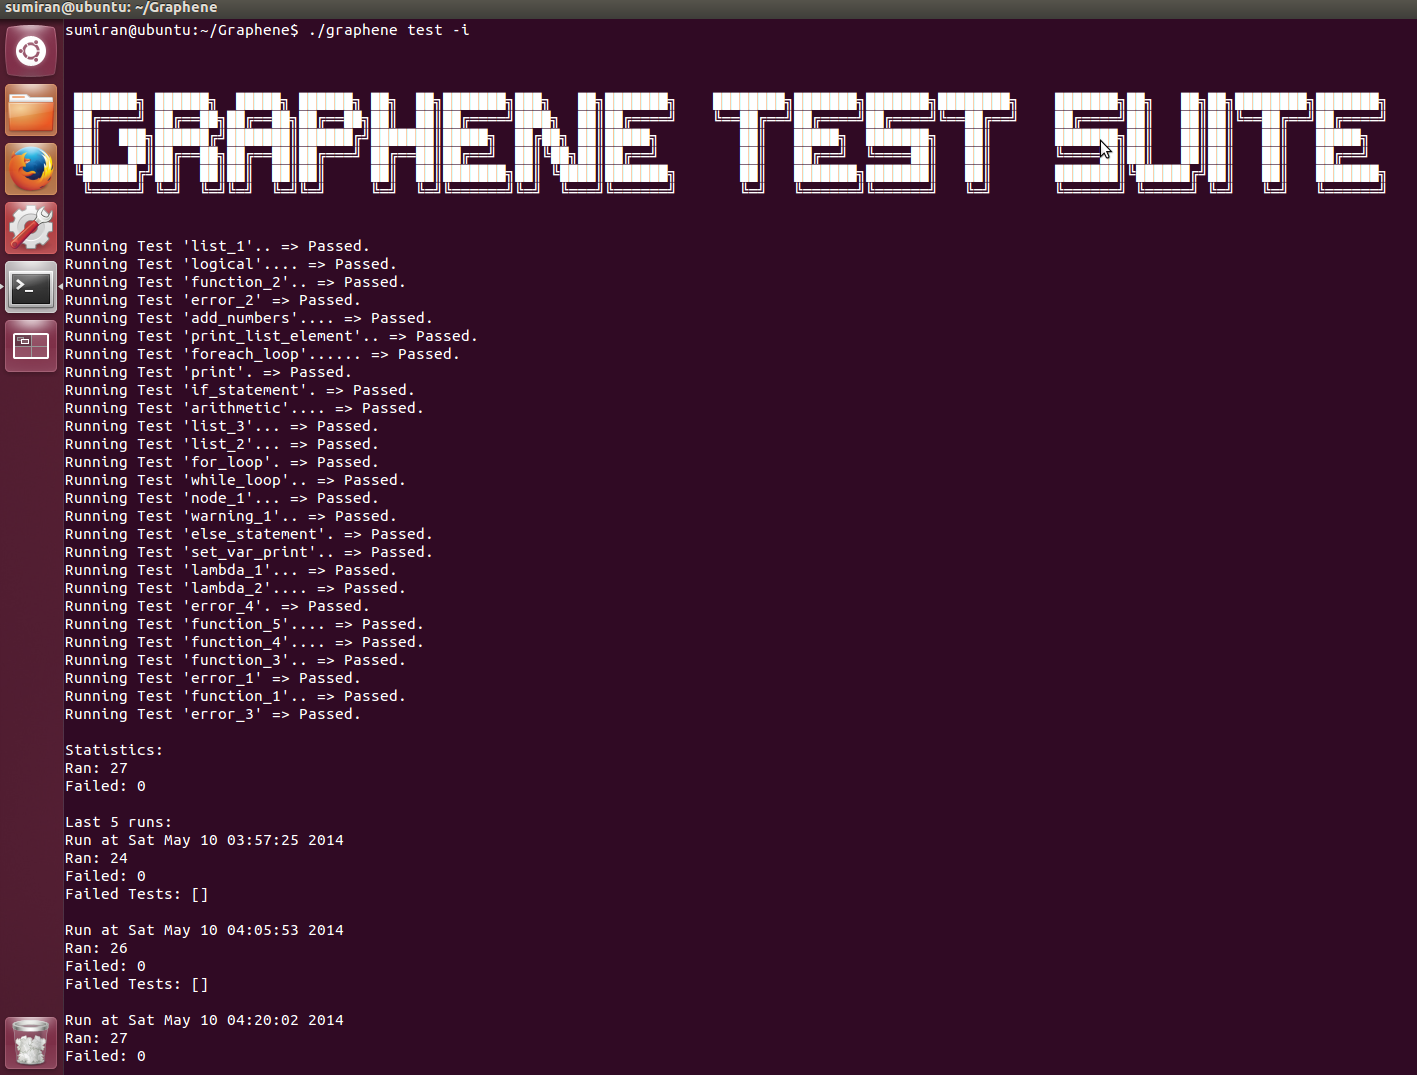
\includegraphics[width=1.2\textwidth]{Tests.png}
\end{figure}

\subsection{Notable Bugs Encountered}
Graphene allows a graph to be directed or undirected. The keywords $d$ and $u$ are used to distinguish between these two types of graphs. Using these keywords however restricted them as use as identifiers. However, since we anticipated that the users will have a tendency to use them as identifiers, we modified these keywords to $d\{$ and $u\{$ respectively as their usage in Graphene are always followed by $\{$.\\

\noindent One of the bugs that we faced was that in Graphene, the function parameters are passed by reference and not by value. We tried to fix this issue but it required a major fix which was not feasible at this point so we tried to make it work with the call by reference.\\


\newpage
\section{Conclusions}
\subsection{Lessons Learned as a team}
We were a team with varying technical backgrounds and different interests. When we took over 3 weeks to decide on a language, hoping to finish on time seemed an uphill task. But, with the right attitude, we learnt that working as a team is a very enriching experience and with an open mind, there is always something to learn from everyone.\\
We learnt the usefulness of git. With a strict rule of no code sharing over any other medium, and a steady ramp up on learning to merge conflicts and merging branches, there were never any WTFs.\\
We learnt the importance of programming to interfaces rather than programming to implementations. There are few things in the world that suck more than having to rewrite perfectly working code.\\
We learnt that locking down spcifications early and nipping potential problems in the bud is very important. Unfixed errors can snowball into major problems that require expensive fixes down the line.
We learnt that having your project scope well defined and achievable is important. As we sit down to write the final project report and we refer back to our original whitepaper and the dreams we saw of our language when we were young and foolish, we realize how different times have turned out to be, for better or for worse. To achieve a stable, complete and robust implementation we had to tradeoff certain dream features.\\
Finally, we learnt that no team is complete without good chemistry between its members. Friendly competitions on the funniest commit messages (that still remain informatory!) kept us alive and interested even during the death phases.\\
In all, if we could go back in time to do it all over again, there are only a few things that we would want to do differently.\\
\subsection{Lessons Learned individually}
\subsubsection{Adith Tekur}
If you're reading this, you've probably read many like this. There are a lot of things other reports will tell you, what to do, and more importantly, what not to do! 

If there’s something I have learnt through all of this, through frustrations and elations, is that there is always a better way to do something. The only question is, are you strong enough to keep at it, long enough to see it through? I have come to realize a lot about the software engineering experience. At the end of the day, it’s about bringing together a group of ordinary people to make something extraordinary!

If this was too philosophical, here come my peers, to give you something more practical to think about.


\subsubsection{Pooja Kalpana Prakash}
My list of take-aways from this project -
\begin {enumerate}
\item "Start early" - easier said than done! In the beginning, it is most likely that you are clueless on where to begin and what to do. Talk to the Professor and the TAs to get some perspective and pointers.
\item Choosing a language all the team members are comfortable with helps a lot. Be there to help each other and most importantly, when in need, ask for help and do it early
\item Laying out everything on paper (a black board in our case!) really helps clarify ambiguities. So leaving your laptop and going the good old pen and paper way may not be a bad idea after all!
\item Getting the entire team to sit together to work is not as easy as it sounds! Make a schedule and stick to it. Make sure to complete all defined milestones. Keep the kernel small and prioritize the features you want to implement. So plan, and plan well.
\item Regression testing is important. You never know what new changes will break your program flow. So start writing test cases early on and incrementally add more.
\item Divide the work well so that different chunks of the kernel can be worked on in parallel. Versioning becomes important, GitHub to the rescue. 
\item Be prepared to debug. And be prepared to debug a lot more!
\end{enumerate}
\subsubsection{Neha Rastogi}
In the start, it seemed like such an impossible task to design a new language and build a compiler for it but we finally did it.
And I think that the credit for that goes to my awesome team. They worked so hard that it motivated me also to at least try to work hard.
Although I have had industry experience in software engineering but it was the first time that I was working on such a complex project. I learned a lot of little things during the course of project, a major one was how to use Github.I had some prior experience with some other version control software like Perforce but Github was a lot different. I tried to use the UI but later resorted to the shell commands.

One other important thing which I learned was Python. I had a lot of experience with C++ but Python was almost new to me. I had some weird encounters during this learning phase (things which were totally different from C++) - I learned that all the objects in Python are static. Since there is no IDE for Python which goes even near to the likes of Visual Studio for C++, I had a really hard time debugging the code by putting print commands at every point. But at the same time, I also got to know some of the amazing features of python like the ease of using lists, dictionaries and other complex data types and one of the most important feature was ducktyping.

\subsubsection{Sarah Panda}
During the course of this project, there are a number of things I started to value more than before. I learnt immensely the evolution of languages and the careful considerations one must make in tradeoffs between efficiency and solid implementations, between features and deadlines, between a beautiful syntax and ability to write beautiful code as a developer. Building a compiler is one of the most exciting challenges of computer science. Here are few of my takeaways from the project:

1. Having a big team has its own pros and cons.  Communication of ideas, ensuring correct execution, and resolving dependencies becomes difficult, if not handled well by someone.  I started to appreciate the role of project manager in a domain heavy software development project.

When done properly, when everyone in the team are in sync and focused, I observed things to work much faster.

2.       It is always good to modularize the code, for both, ease of understanding and isolating failures. It saved a lot of energy in debugging during the end phases.

3.       Regression testing is a vital element of development lifecycle.  Without it, some or the other change would silently break an existing functionality and it would remain unknown for long.

4.       Change in grammar at a later point in time can be have bigger implications, i.e. could break functionality. So, it is better to ensure any conflicts are removed well in advance and the language specifications are locked down, to avoid changing the grammar at a later point.

5.       Lastly, it is ok to make the above mistakes during the project. To err is human.
\subsubsection{Sumiran Shah}
I learnt that good software is not written from good code, but from good design. What I think worked well for us was that we planned interfaces and end to end flows in advance before sitting down to work. Following good development practices helped minimize the overhead incurred due to many people working on the same code. Liberal use of Git, Flowdock and WhatsApp to collaborate definitely helped.
I also learnt the importance of automating test cases and the effort it saves in the long run. Ofcourse, my main takeaway would be learning to constantly focus on the big picture and not get lost in small optimizations.
\\
\\
Working on Graphene made me realize how much I take modern language compilers for granted. Developing a programming language is as much an art as it is a science. All programming languages being Turing complete can be argued to technically be the same.
What sets a language apart is the ease of use and the ability of the developer to focus on his problem statement, and not on technicalities of the language. I learnt how Python does exactly this and we tried to implement Graphene with a similar idea in mind.
\newline

\subsection{Advice for future teams}
Don't aim to begin early and assume that will work itself out. Work always expands to fit all the time it has available. Instead, aim to end one week before the deadline. Be rigorous in coding standards but flexible in implementation as requirements might change. Make sure you frequently meet your TA/mentor and professor Aho for feedback and to ensure you are on the right track. Above all, enjoy the experience. Writing a compiler will probably be the most satisfying project you will have ever undertaken in your CS careers.

\newpage
\section{Appendix}
\subsection{Git History}
\begin{verbatim}
commit 085e224b5fe3201a61797517011cb1394b7715a4
Author: Sumiran <srs2222@columbia.edu>
Date:   Sun May 11 09:15:19 2014 -0400

    We're live! So long and thanks for all the code!

commit ac3c361d25e5f863f218a3cfc347e6a4e688bf3d
Merge: 738462e ac3c361
Author: Sumiran <srs2222@columbia.edu>
Date:   Sun May 11 09:13:15 2014 -0400

    Merge conflicts

commit 738462eb56b229e1966b9f54802585ee03d5ee3e
Author: Adith Tekur <at2904@columbia.edu>
Date:   Sun May 11 07:40:03 2014 -0400

    Fixed bash, UI who element and graph declaration on key

commit 6525c8a02b53bded2ef493a4d825c28989d94616
Author: Adith Tekur <at2904@columbia.edu>
Date:   Sun May 11 02:43:59 2014 -0400

    edge addition! powered by nodelookup™

commit a210a522d109506192944af991a658441b32ff76
Merge: 95f2e19 7161006
Author: Adith Tekur <at2904@columbia.edu>
Date:   Sun May 11 01:45:02 2014 -0400

    Merge into master after Assets

commit 95f2e19ac9976ef86bd9bd5260d41eab4446003b
Merge: 66ee79d 051ed13
Author: Adith Tekur <at2904@columbia.edu>
Date:   Sun May 11 01:42:06 2014 -0400

    Fixed UI, nodeLookup, overlay. Also, I see through you!

commit 7161006117d0d3967a8d2e11269ff934d1103844
Author: sumiran <srs2222@columbia.edu>
Date:   Sun May 11 00:03:44 2014 -0400

    No Comments. Ok. Maybe we do now.

commit f24b9c7541d9ffa6aff5873aa2a2133ec2d12d19
Author: Sumiran <srs2222@columbia.edu>
Date:   Sat May 10 21:22:27 2014 -0400

    Presentation slides, format sample .ene code

commit 66ee79d7e2d1c5fde49b4cafd2a6242b832dc786
Author: Adith Tekur <at2904@columbia.edu>
Date:   Sat May 10 06:29:14 2014 -0400

    You get a profile! And You get a profile! Everyone gets a profile!

commit 051ed133f967b6d4f219a8ce66b1ca313c317434
Merge: eaa24fa 0993a93
Author: Sarah Panda <sp3206@columbia.edu>
Date:   Sat May 10 04:36:04 2014 -0400

    Cluster this\!\!

commit 0993a93d18d2bc86fc49d9877093f63358fce58a
Merge: 47b1b0a 149cc94
Author: Pooja Prakash <poojamaiya@gmail.com>
Date:   Sat May 10 04:23:52 2014 -0400

    Testing times

commit 47b1b0a88ff0d7003b8ca045757275ce5a1a981a
Author: Pooja Prakash <poojamaiya@gmail.com>
Date:   Sat May 10 03:31:24 2014 -0400

    just one more test case! :X

commit eaa24fa60cb37df254d00e09bcbeb944ea3e4d4c
Author: Sarah Panda <sp3206@columbia.edu>
Date:   Sat May 10 02:33:13 2014 -0400

    added clustering with lambda, also goutput

commit 120f23dfec46a5eb2f3abfdd1b951d26a46862d3
Author: Pooja Prakash <poojamaiya@gmail.com>
Date:   Sat May 10 02:10:24 2014 -0400

    Added ';' at the end of selectionstatement and iterationstatement productions; 
    Fixed functions to deal with more than 2 args; Added a few test-cases

commit 149cc946874fcb0906da73e94fb6499562ac520d
Author: Sumiran <srs2222@columbia.edu>
Date:   Sat May 10 01:27:41 2014 -0400

    HOLD IT! WE FORGOT THE MODULO

commit e58a9007050a37cef102bf729c3e5579948a97e3
Author: Sumiran <srs2222@columbia.edu>
Date:   Fri May 9 20:32:35 2014 -0400

    FOREACH works again. Grrr

commit dd7930bb3e167f808b8611144aea524a0628f589
Merge: bd76b0b f9cb8fc
Author: Sumiran <srs2222@columbia.edu>
Date:   Fri May 9 20:30:23 2014 -0400

    Merge branch 'master' of github.com:Adith/Graphene

commit bd76b0bf323f578ef168977e62036001b97bfb2e
Author: Sumiran <srs2222@columbia.edu>
Date:   Fri May 9 20:23:47 2014 -0400

    Made FOREACH work again. Grrrrr

commit 96e9f003fefe5be5e651041a86f164e349782471
Author: Adith Tekur <at2904@columbia.edu>
Date:   Fri May 9 07:56:34 2014 -0400

    added random person UI profile handler

commit 4c2563f60acef5b8cd78c2fcaaeb6f712a9ef1b8
Author: Pooja Prakash <poojamaiya@gmail.com>
Date:   Fri May 9 05:46:32 2014 -0400

    Support for list element as argument into function added; 
    Productions for True & False added; Resolved all reduce-reduce conflicts; 
    while loop modified to take conditions based on True & False; 
    Fixed if to work only on True (instead of anything but 0); 
    Error handling - number of function argument mismatch, invalid function

commit f9cb8fc048c80664c4be4e7a11599258fe8b9aed
Author: Sarah Panda <sp3206@columbia.edu>
Date:   Fri May 9 02:06:11 2014 -0400

    node property retreival, lambda as argument

commit f348919d01a56facd15e7bc091a002518f02f358
Author: Pooja Prakash <poojamaiya@gmail.com>
Date:   Fri May 9 01:32:06 2014 -0400

    expressions for function arguments and return values added; productions for True, 
    False added; fixed while loops; line numbers for error outputs;

commit cc0f1dbb971aa597fb8bd7c4a2bad254ac55b1d7
Author: Sumiran <srs2222@columbia.edu>
Date:   Thu May 8 23:32:13 2014 -0400

    LAMBDAAAAAA! Can pass lambdas as arguments to functions

commit f763935a1a0a96794d4c6182750f44df6278a9dc
Author: Pooja Prakash <poojamaiya@gmail.com>
Date:   Thu May 8 03:02:42 2014 -0400

    logical or working; keyboard interrupt handled; work in progress - error handling

commit 43ef679ab950456793c17ac926f51f37c69ec22e
Author: neharastogi <nr2477@columbia.edu>
Date:   Wed May 7 12:45:06 2014 -0400

    Removed shift reduce conflicts by adding precendences

commit 126861b19fc43c96ca00d972080bfe3d4c9454ab
Author: Sarah Panda <sp3206@columbia.edu>
Date:   Wed May 7 00:57:15 2014 -0400

    Lambda basics

commit 274ecc71b5e746a6d2611d8722ae2b485de1354c
Author: Sarah Panda <sp3206@columbia.edu>
Date:   Tue May 6 23:46:28 2014 -0400

    Moved evaluateAST to lib/ast

commit afa51c71e5b5856ad039c80934881d7c550ee903
Author: Adith Tekur <at2904@columbia.edu>
Date:   Wed Apr 30 01:15:06 2014 -0400

    Overlay, evaluateAST partly cleaned up

commit 2e1619699703023a5e35fd9a1a94347ae57a8e1e
Merge: 8a470c7 19c5787
Author: Adith Tekur <at2904@columbia.edu>
Date:   Tue Apr 29 02:11:50 2014 -0400

    Fixed end-to-end, added sample, foreach now processes expression

commit 19c5787913d98db6e7ab37ef5ce9903f99df7438
Author: Pooja <poojamaiya@gmail.com>
Date:   Mon Apr 28 05:24:17 2014 -0400

    fixed multi-line pgms; added src file support

commit 8a470c74e37ffc79fe4ba2e5e68d6c5e3ec7470b
Author: Pooja <poojamaiya@gmail.com>
Date:   Sun Apr 27 22:49:11 2014 -0400

    handled multi-line programs

commit 3c081163770fd7807178dfe4a9fc95b845945f6e
Author: Sarah Panda <sp3206@columbia.edu>
Date:   Sun Apr 27 21:25:57 2014 -0400

    dataset and visualization support

commit b6d0f5d2844f1419b298d83a7b475edf09ecf92b
Merge: c325e8f f7609f7
Author: Adith Tekur <at2904@columbia.edu>
Date:   Sat Apr 26 03:03:52 2014 -0400

    Knock Knock! Who's there? Function! Function who?! Function Chaining!

commit c325e8fb2e5e0f9270cd3767d446652b41aca99b
Merge: 3129990 2afac43
Author: Adith Tekur <at2904@columbia.edu>
Date:   Fri Apr 25 00:16:48 2014 -0400

    Merge branch 'master' of github.com:Adith/Graphene
    merge

commit 31299906c87b990820ca03e1a31a9cff9e86b898
Author: Adith Tekur <at2904@columbia.edu>
Date:   Thu Apr 24 06:34:22 2014 -0400

    Added callchain

commit 2afac43a46d0797dfcfc0928276e142365a55f11
Author: Pooja Prakash <poojamaiya@gmail.com>
Date:   Thu Apr 24 06:34:05 2014 -0400

    Support for negative numbers; List assignments of the form - a[i]=b

commit e05a96f106c936a5b9b8369d1578e9eaf1cbc3cc
Merge: 9332410 130aa04
Author: Pooja Prakash <poojamaiya@gmail.com>
Date:   Thu Apr 24 04:57:00 2014 -0400

    list functions - length(), append() implemented; 
    assignments using array indices of the form b = a[i] supported

commit 9332410ae3570210921d362de33b623ba41507bc
Author: Pooja Prakash <poojamaiya@gmail.com>
Date:   Thu Apr 24 04:48:36 2014 -0400

    list functions - length(), append() implemented; 
    assignments using array indices of the form b = a[i] supported

commit 130aa045bfab590461b0d5a2a16018f20d83cb4c
Merge: 79f2cd5 d69211d
Author: Adith Tekur <at2904@columbia.edu>
Date:   Thu Apr 24 04:34:45 2014 -0400

    Merge branch 'master' of github.com:Adith/Graphene
    merge

commit 79f2cd58b830a3127a6add04a24aceea5c6fb1f2
Author: Adith Tekur <at2904@columbia.edu>
Date:   Thu Apr 24 04:34:14 2014 -0400

    Added getNodes, nodelookup

commit f7609f7de934e06a57f6f0b521d4735b56cda51f
Author: Sumiran <srs2222@columbia.edu>
Date:   Thu Apr 24 02:36:24 2014 -0400

    Added variable scoping in compound statements (statement blocks)

commit bf3bc394d75576132bcc34fd8b89f07dc41feca7
Author: Sumiran <srs2222@columbia.edu>
Date:   Thu Apr 24 01:08:57 2014 -0400

    Foreach loops and stuff

commit d69211da6eb7fc52cccedfc0f90afcfd9924c7ed
Merge: 2688c6b ec90740
Author: Pooja Prakash <poojamaiya@gmail.com>
Date:   Wed Apr 23 22:17:35 2014 -0400

    merged into master

commit 2688c6b76bf51fc2c5b095105bcc1160d2643a91
Author: Adith Tekur <at2904@columbia.edu>
Date:   Wed Apr 23 21:41:21 2014 -0400

    Added node removal, getAdjacent, member funcation call

commit ec90740117b1df224df979ebc8f60e224ba408de
Author: Pooja Prakash <poojamaiya@gmail.com>
Date:   Wed Apr 23 21:35:37 2014 -0400

    support for empty lists implemented

commit 6536e9d566ea76511dca2822d496bac2145e6a54
Author: Pooja Prakash <poojamaiya@gmail.com>
Date:   Wed Apr 23 20:00:00 2014 -0400

    support for lists of lists implemented

commit 0428884daa31f2ff45cb7144208754876424ce4a
Author: Pooja Prakash <poojamaiya@gmail.com>
Date:   Wed Apr 23 17:57:30 2014 -0400

    fixed assignments, basic lists work, lists of lists in progress

commit 0d691a918039b6a94714169851168c73b372fd22
Merge: 07a829b 96b1afd
Author: Adith Tekur <at2904@columbia.edu>
Date:   Tue Apr 22 03:19:31 2014 -0400

    merge after call stack update and updated gitignore

commit 07a829bc47b667a352ca15239159cfc3059ff53d
Author: Adith Tekur <at2904@columbia.edu>
Date:   Tue Apr 22 03:06:43 2014 -0400

    Added call stack

commit 96b1afd037dae484df398f3f1dde1e4057aa90d1
Author: neharastogi <nr2477@columbia.edu>
Date:   Mon Apr 21 19:17:50 2014 -0400

    If-else added and relational operators

commit e4b73992f48afc6f97a6b50ff99ee45dd9f0a533
Author: Sarah Panda <sp3206@columbia.edu>
Date:   Mon Apr 21 02:03:22 2014 -0400

    add edges to a graph

commit 5ec9b4597ad7c33ac3dc9891acc74f7a878dd278
Author: Pooja Prakash <poojamaiya@gmail.com>
Date:   Sun Apr 20 23:19:50 2014 -0400

    Fixed I/O path

commit fce4e7854bd751c24fff39728d4dfb00f4e3d608
Author: Pooja Prakash <poojamaiya@gmail.com>
Date:   Sun Apr 20 07:15:48 2014 -0400

    Fixed UI I/O path

commit eafb3ccd7fb93f15f853d9cbb276cad1f125cb94
Author: Sarah Panda <sp3206@columbia.edu>
Date:   Sun Apr 20 04:40:38 2014 -0400

    Fixed func_call, func_args and func_ret_values

commit 80f30ca4ef5f784e0778f4601f2164dd02ee2e39
Author: Adith Tekur <at2904@columbia.edu>
Date:   Sun Apr 20 04:18:57 2014 -0400

    Fixed func_call, func_args and func_ret_values

commit 248dcac67574a6680836022fa8049618fe08c9ab
Author: Adith Tekur <at2904@columbia.edu>
Date:   Sat Apr 19 21:47:31 2014 -0400

    Fixed test bug

commit 4a367c97e6cf516b60602eaf772d4f78e070640c
Author: Adith Tekur <at2904@columbia.edu>
Date:   Thu Apr 17 04:31:54 2014 -0400

    Updated test infra

commit 6415239ef916bbbd35e89bd1d9355796be82d07d
Author: Pooja Prakash <poojamaiya@gmail.com>
Date:   Thu Apr 17 01:39:15 2014 -0400

    Support for functions with arguments implemented

commit 3020d62039623bdcac8eac14cbdef046b7832823
Author: Adith Tekur <at2904@columbia.edu>
Date:   Wed Apr 16 23:55:03 2014 -0400

    Testing framework up

commit 4d076eebad79f76a38d6c7ebbdc6f7c196b76cdf
Author: Pooja Prakash <poojamaiya@gmail.com>
Date:   Wed Apr 16 01:42:22 2014 -0400

    user defined func arglist+returnlist scaffolding

commit 1f0da704b7b60aeeb9178c72256afa241da9f6e8
Merge: 58316e0 da72052
Author: Adith Tekur <at2904@columbia.edu>
Date:   Tue Apr 15 22:59:38 2014 -0400

    Merge branch 'master' of github.com:Adith/Graphene
    merge

commit 58316e015bba8c22c7f9f552d58e94c764de3dcd
Author: Adith Tekur <at2904@columbia.edu>
Date:   Tue Apr 15 22:59:07 2014 -0400

    get_data support

commit da720525b1adb9910cafa9ab44d6a8217330f580
Author: Sumiran <srs2222@columbia.edu>
Date:   Tue Apr 15 19:22:38 2014 -0400

    For loops are born

commit e35ecd1e3aa3ed83ee54c3c50daf02bb35199656
Author: Adith Tekur <at2904@columbia.edu>
Date:   Tue Apr 15 08:12:45 2014 -0400

    Graph infra up. Default edge keys have to be added. Default Node reference by ID.

commit ccb7a6e95ff3ba6b458b398a5d79b9eb6d805543
Author: Adith Tekur <at2904@columbia.edu>
Date:   Tue Apr 15 01:27:19 2014 -0400

    Node data structure implemented

commit 54aff234498ce9731824b6a9632ac0ea7c45648a
Author: Adith Tekur <at2904@columbia.edu>
Date:   Sat Apr 12 08:12:49 2014 -0400

    Added node object handlers

commit 6244ea83bbd337111a01dc989cc9b4df4b16edce
Author: Adith Tekur <at2904@columbia.edu>
Date:   Sat Apr 12 02:48:07 2014 -0400

    Added Node scaffolding

commit ff4990d2905514e20202e5b1f0f32d3a17c404a0
Author: Adith Tekur <at2904@columbia.edu>
Date:   Sat Apr 12 02:10:23 2014 -0400

    Logger up and running, scaffolding for setup is up.

commit 04f68a86c2b038a783d4cd6308c62cd30617007e
Author: Pooja Prakash <poojamaiya@gmail.com>
Date:   Fri Apr 11 22:19:57 2014 -0400

    fixed input(), started Node etc.

commit 357f97f17b89ac073e789232d777a41f91e5a346
Author: Pooja Prakash <poojamaiya@gmail.com>
Date:   Fri Apr 11 03:49:49 2014 -0400

    Fixed regression input() bug

commit 6ad04d2c71ab6dc91bb83592cedd2323e7c77a9a
Merge: 7f4cd84 5a273e2
Author: Pooja Prakash <poojamaiya@gmail.com>
Date:   Fri Apr 11 03:20:39 2014 -0400

    Merge-O-Rama! Regression bug: Input doesn't work because fn call 
    now needs a node obj trampoline

commit 7f4cd840b2f733c74a651a37791ceabd3a6bf312
Author: Pooja Prakash <poojamaiya@gmail.com>
Date:   Fri Apr 11 03:05:13 2014 -0400

    pooja commit before merge

commit 5a273e2a2538af5ebb12a082d7e9411ec2591e2c
Author: Adith Tekur <at2904@columbia.edu>
Date:   Fri Apr 11 03:02:43 2014 -0400

    A little cleanup, Merge into master

commit 2c359a2c008c5e9a2288f76923761ff0ae97808e
Author: Pooja Prakash <poojamaiya@gmail.com>
Date:   Fri Apr 11 01:59:31 2014 -0400

    Debug, variable handling, symbol table, AST nodes extended

commit 8cb00973ca266909ef9d1be8f7c1d557ac526f73
Author: Pooja Prakash <poojamaiya@gmail.com>
Date:   Fri Apr 11 00:14:58 2014 -0400

    Support for while. TODO: work on the expression part of while in 
    the evaluateAST() once relational operators are supported

commit 891377e3d179a1acee74cce260b88608c10566e0
Author: Adith Tekur <at2904@columbia.edu>
Date:   Tue Apr 8 03:13:49 2014 -0400

    Added State snapshot in UI render path. Commit fixes Issue #2

commit 0d9565d860c28085317a2c6257ba0e0f73166db5
Author: Adith Tekur <at2904@columbia.edu>
Date:   Mon Apr 7 23:41:34 2014 -0400

    I/O fastpath up and running. Issue #1 closed.

commit 8bc87bbef72096dcea2903b8ba7f3bcd607bd171
Author: Pooja Prakash <poojamaiya@gmail.com>
Date:   Mon Apr 7 19:00:42 2014 -0400

    handled whitespace; modified p_call() production; included mapping for exit function

commit ccc327b8e028c84dc1e0e3b4d86696775f984cde
Author: Pooja Prakash <poojamaiya@gmail.com>
Date:   Mon Apr 7 18:46:30 2014 -0400

    Pooja's dev branch

commit 4dd793187205bcd78e2b7c4b52cd3613298bddbb
Author: Adith Tekur <at2904@columbia.edu>
Date:   Mon Apr 7 04:58:35 2014 -0400

    OO Scaffolding up

commit 6eeebf13e8add84383f24b9544432b4a2038e825
Author: Adith Tekur <at2904@columbia.edu>
Date:   Sun Apr 6 23:02:48 2014 -0400

    Fixed missing attributes

commit 3429e013146bddb46369b1f753b38f2f9bbfa00f
Author: Adith Tekur <at2904@columbia.edu>
Date:   Sun Apr 6 22:53:41 2014 -0400

    Completed GUI Scaffolding

commit 37a1f2828e453a3f7ca360e39f69bfeb23289ba9
Merge: 0957376 8a7727a
Author: Adith Tekur <at2904@columbia.edu>
Date:   Sun Apr 6 16:48:37 2014 -0400

    GUI merge

commit 09573762abd0d9eeff89c1a1eda5c1a76939af34
Author: Adith Tekur <at2904@columbia.edu>
Date:   Sun Apr 6 16:27:30 2014 -0400

    Added GUI scaffolding

commit 8a7727a0febd8f2c3aba43f02d72489161efeed1
Author: sarahpanda <sp3206@columbia.edu>
Date:   Sun Apr 6 03:47:37 2014 -0400

    added multiple expressions, assignment(see desc)
    
    Multiple statements are handled. in command line u enter multiple 
    statements separated by ;
    
    example execution:
    graphene> x=2.1+3.2;print(x);print("HelloWorld");
    
    Newline isnt added yet. Will add soon.

commit b49b1a14d7a6cc1524a747f9930d44ac0c46ca96
Author: Sumiran Shah <sumiranshah@gmail.com>
Date:   Sat Apr 5 19:10:18 2014 -0400

    More beautiful syntax error message

commit b9a1a06d805dfa903d488fa7e6124537b5db15a7
Merge: cdd98a7 b90b4ab
Author: Sumiran Shah <sumiranshah@gmail.com>
Date:   Sat Apr 5 18:50:12 2014 -0400

    Merge branch 'master' of ssh://github.com/Adith/Graphene

commit cdd98a77a6e2ba278daea8062c2d94779713cb1d
Author: Sumiran Shah <sumiranshah@gmail.com>
Date:   Sat Apr 5 18:49:50 2014 -0400

    Functions can now take entire arglists. Also displaying a less 
    aggressive function-not-found message.

commit b90b4ab74b0cc0ed6100f97b93389693d66f81a3
Author: neharastogi <nr2477@columbia.edu>
Date:   Sat Apr 5 17:36:45 2014 -0400

    Function for output Nodes

commit 018f4bbd8c92b4484a716550344076abce184415
Author: sarahpanda <sp3206@columbia.edu>
Date:   Sat Apr 5 17:24:24 2014 -0400

    Input to Out and Out to Input format conversion

commit 310e0109f6db9a5ebebb1bec8f1887e6ecd540ca
Author: Sumiran Shah <sumiranshah@gmail.com>
Date:   Sat Apr 5 16:38:32 2014 -0400

    Added initial Graph internal data type representation

commit 3b44e56596d7d868212ee391628a74bef15bd716
Author: Sumiran Shah <sumiranshah@gmail.com>
Date:   Sat Apr 5 15:04:13 2014 -0400

    Added gitignore for .pyc and .out

commit 3f379b2dbe0047f023055e10ef7604e925ad5bdb
Author: Adith Tekur <Adith@users.noreply.github.com>
Date:   Sun Mar 30 19:40:59 2014 -0400

    Update README.md

commit 0a5add1382cd7250557179c4181ca44d12112f9a
Author: Sumiran Shah <sumiranshah@gmail.com>
Date:   Sun Mar 30 19:06:39 2014 -0400

    Hello World with function mapping

commit 1b5a202a6ffe592ec16b2998c388e7b2e408970b
Author: Sumiran Shah <sumiranshah@gmail.com>
Date:   Sun Mar 30 18:48:36 2014 -0400

    Hello World

commit 4b1b9f1798fb01c68f79b7e8c7278031786dc2bb
Author: Adith Tekur <at2904@columbia.edu>
Date:   Wed Mar 26 11:48:46 2014 -0400

    Ref Manual and Tutorial

commit bd0567465508726e7911cff4918a53354e3c6455
Author: Adith Tekur <at2904@columbia.edu>
Date:   Mon Mar 24 04:44:53 2014 -0400

    LRM draft

commit 9380149e6c6ebd985eb2e8cce1fbb4306f28ea40
Author: Adith Tekur <at2904@columbia.edu>
Date:   Sun Mar 16 21:45:11 2014 -0400

    Added Proposal

commit 2c8e0c7f9c2f2fc9dcab69a3a298c816e29287cc
Author: poojamaiya <poojamaiya@gmail.com>
Date:   Sat Feb 22 16:36:44 2014 -0500

    Updated details on initial operators list

commit 0022499a6750c2b9f50d7819a2e9f1d7d9e21ca4
Author: poojamaiya <poojamaiya@gmail.com>
Date:   Sat Feb 22 14:46:39 2014 -0500

    Whitepaper v1.0
    
    Basic data-types, functionalities, etc.

commit 3638400b5cd32f4e6073018de95d7ba4b295c2dd
Author: Adith Tekur <Adith@users.noreply.github.com>
Date:   Fri Jan 24 16:39:03 2014 -0500

    Create README.md

\end{verbatim}
\subsection{Code}
\subsubsection{Graphene Main: graphene.py}
 
\begin{verbatim}
#! /usr/bin/env python

import ply.yacc as yacc
import ply.lex as lex
import os, sys
if os.name == "posix":
    import readline
import inspect
sys.path.append(os.path.dirname(os.path.realpath(__file__)))

from itertools import chain
import itertools
import sys
import types
import decimal
from lib import grapheneLib as lib
from lib import grapheneHelper as helper
from lib import ast
from collections import namedtuple
import logging

# import symboltable

fread = False
logger = logging.getLogger()
lineNo = 0;

if len(sys.argv) > 1:
    if "-d" in sys.argv:
        logger.setLevel(logging.DEBUG)
    elif "-i" in sys.argv:
        logger.setLevel(logging.INFO)
    if "-f" in sys.argv:
        fread = True


NumberTypes = (types.IntType, types.LongType, types.FloatType, types.ComplexType)

errorDict = {'ID':'id', 
    'LPAREN':'\'(\'', 
    'DEF':'\'def\'', 
    'IMPLY': '\'=>\'', 
    'LAMDA':'\'lambda\'', 
    'RPAREN':'\')\'', 
    'STRING': 'string',
    'SQRBEGIN':'\'[\'', 
    'SQREND':'\']\'', 
    'CURLBEGIN':'\'{\'', 
    'CURLEND':'\'}\'', 
    'NUMBER': 'number',
    'IF':'\'if\'', 
    'ELSE':'\'else\'', 
    'COMMA':'\',\'',  
    'GR':'\'>\'', 
    'LS':'\'<\'', 
    'NODE':'\'NodeType\'', 
    'GRAPH':'\'Graph\'',
    'GRAPHTYPE':'\'d\', \'u\'', 
    'CONNECTOR':'\'->\', \'<->\'', 
    'NEW':'\'new\'', 
    'NEWLINE':'\'\\n\'', 
    'DOT':'\'.\'', 
    'WHILE':'\'while\'', 
    'FOR':'\'for\'', 
    'FOREACH':'\'foreach\'', 
    'IN':'\'in\'', 
    'HAS':'\'has\'', 
    'ON':'\'on\'', 
    'COLON':'\':\'', 
    'GRTEQ':'\'>=\'',
    'LESSEQ':'\'<=\'',
    'EQUAL':'\'=\'',
    'NEQUAL':'\'!=\'',
    'LOGAND':'\'&&\'',
    'LOGOR':'\'||\'', 
    'ADD_STORE':'\'+=\'', 
    'REMOVE_STORE':'\'-=\'',
    '=':'\'=\'',
    ';':'\';\'',
    '+': '\'+\'',
    '*': '\'*\'',
    '-': '\'-\'',
    '/': '\'/\'',
    '%': '\'%\''}

tokens = ('ID', 'LPAREN', 'DEF', 'IMPLY', 'LAMDA', 'RPAREN', 'STRING', 'SQRBEGIN', 
'SQREND', 'CURLBEGIN', 'CURLEND', 'NUMBER', 'IF', 'ELSE', 'COMMA', 'GR', 'LS', 'NODE', 
'GRAPH','GRAPHTYPE', 'CONNECTOR', 'NEW', 'NEWLINE', 'DOT', 'WHILE', 'FOR', 'FOREACH', 
'IN', 'HAS', 'ON', 'COLON', 'GRTEQ','LESSEQ','EQUAL','NEQUAL','LOGAND','LOGOR', 
'ADD_STORE', 'REMOVE_STORE','TRUE','FALSE')
literals = [';', '=', '+', '-', '*', '/', '%']

t_GR = r'\>'
t_LS = r'\<'

RESERVED = {
  "def": "DEF",
  "if": "IF",
  "else": "ELSE",
  "return": "RETURN",
  "while": "WHILE",
  "for": "FOR",
  "foreach": "FOREACH",
  "in":"IN",
  "has": "HAS",
  "on": "ON",
  "NodeType": "NODE",
  "Graph": "GRAPH",
  "Edge": "EDGE",
  "d{": "GRAPHTYPE",
  "u{": "GRAPHTYPE",
  "->": "CONNECTOR",
  "<->": "CONNECTOR",
  "lambda": "LAMDA",
  "True":"TRUE",
  "False":"FALSE"
  }

t_IMPLY = r'=>'

t_CURLBEGIN = r'{'

t_CURLEND = r'}'

t_SQRBEGIN = r'\['

t_SQREND = r'\]'

t_DOT = r'\.'

t_COLON = r':'

t_GRTEQ = r'\>='

t_LESSEQ = r'\<='

t_EQUAL = r'\=='

t_NEQUAL = r'\!='

t_LOGAND = r'\&&'

t_ADD_STORE = r'\+='

t_REMOVE_STORE = r'-='

t_LOGOR = r'\|\|'

t_LPAREN = r'\('

t_RPAREN = r'\)'

t_STRING = r'[\"\'][a-zA-Z\ /.:0-9(){}]*[\"\']'

t_COMMA = r','

t_NODE = r'Node'

t_GRAPH = r'Graph'

t_NEW = r'new'

t_CONNECTOR = r'<?->'

#t_GRAPHTYPE = r'(d|u){1}'

precedence = (
	('left','LOGAND','LOGOR'),
	('left', 'EQUAL', 'NEQUAL'),
	('left','LS','GR','GRTEQ', 'LESSEQ'),
	('left', '+', '-'),
    ('left', '%'),
	('left', '*', '/'),
)

def t_TRUE(t):
    r'True'
    t.type = RESERVED.get(t.value, "TRUE")
    logging.debug("----- BOOL: "+t.type+" ------")
    return t

def t_FALSE(t):
    r'False'
    t.type = RESERVED.get(t.value, "FALSE")
    logging.debug("----- BOOL: "+t.type+" ------")

def t_GRAPHTYPE(t):
    r'(d|u){1}{'
    t.type = RESERVED.get(t.value, "GRAPHTYPE")
    logging.debug("----- TOKEN: GRAPHTYPE - "+t.type+" ------")
    return t

def t_ID(t):
    r'[a-zA-Z\_][a-zA-Z\_0-9]*'
    t.type = RESERVED.get(t.value, "ID")
    logging.debug("----- TOKEN: ID - "+t.type+" ------")
    return t

def t_newline(t):
    r'\n+'
    t.lexer.lineno += len(t.value)
    t.lexpos += len(t.value)
    t.type = "NEWLINE"
    if t.lexer.paren_count == 0:
        return t

def t_WHITESPACE(t):
    r'\s+'
    t.lexpos += len(t.value)

def t_NUMBER(t):
    r"""(\-?\d+(\.\d*)?|\.\d+)([eE][-+]? \d+)?"""
    #t.value = decimal.Decimal(t.value)
    return t

def t_error(t):
    print "Syntax error:"
    print "Type: ",t.type
    print "Token: ",t.value
    print "Line: ",t.lineno
    print "Column: ",t.lexpos
    sys.exit()

def p_error(p):
    if p is None:
        print "Syntax error: unexpected EOF"
    else:
        print "Syntax error at line {}: unexpected token '{}'".format(p.lineno, p.value)

    #Ugly hack since Ply doesn't provide any useful error information
    import inspect
    frame = inspect.currentframe()

    cvars = frame.f_back.f_locals
    errorOutput = []

    for k in cvars['actions'][cvars['state']].keys():
        errorOutput.append(errorDict[k])
        # print errorDict[k]

    print 'Expected one of: ',', '.join(errorOutput) 
    print '\n'
    # print 'Found:', cvars['ltype']
    # print 'Current stack:', cvars['symstack']
    sys.exit()

lexer = lex.lex();

def p_program(p):
    '''program : declarationlist'''
    logging.debug("----- program ------")
    p[0]=p[1]

def p_declarations(p):
    '''declarationlist : declaration declarationlist
                       | declaration'''
    logging.debug("----- declaration list ------")
    p[0]=p[1]

def p_declaration(p):
    '''declaration : funcdec
                   | vardec'''
    logging.debug("----- declaration ------")
    p[0]= p[1]
    ast.evaluateAST(p[0], lineNo)

def p_vardec(p):
    '''vardec : node-dec ';'
              | graph-dec ';' '''
    logging.debug("----- variable declaration ------")

    p[0] = p[1]

def p_node(p):
    '''node-dec : ID HAS keylist'''
    #Note - keylist implies parameters

    logging.debug("----- Node declaration -----")

    node = ast.ASTNode()
    node.type = 'node-dec'

    child1 = ast.ASTNode()
    child1.value = p[1]
    child2 = ast.ASTNode()
    child2.value = p[3]

    node.children.append(child1)
    node.children.append(child2)
    p[0] = node

def p_keylist(p):
    '''keylist : idOrAlphanum
               | idOrAlphanum COMMA keylist'''

    logging.debug("----- Node declaration keylist -----")

    p[0] = []
    if p[1].type == "id":
        p[0].append(p[1].children[0])
    else:
        p[0].append(p[1].value)
    if len(p) == 4:
        if p[1] in p[3]:
            logging.critical("Same property name for node.")
            system.exit(-1)

        p[0] += p[3]

def p_graph(p):
    '''graph-dec : GRAPH ID HAS GRAPHTYPE edgelist CURLEND
                 | GRAPH ID HAS GRAPHTYPE edgelist CURLEND ON idOrAlphanum '''

    logging.debug("----- Graph declaration -----")

    node = ast.ASTNode()
    node.type = 'graph-dec'

    gid = ast.ASTNode()
    gid.type = "id"
    gid.value = p[2]
    gtype = ast.ASTNode()
    gtype.type = "terminal"
    gtype.value = p[4]
    edges = p[5]

    key = ast.ASTNode()
    key.type = "terminal"
    key.value = "id"

    if(len(p) == 9):
        key.value = p[8]

    node.children.append(gid)
    node.children.append(gtype)
    node.children.append(key)
    node.children.append(edges)

    p[0] = node


def p_edgelist(p):
    '''edgelist : idOrAlphanum CONNECTOR idOrAlphanum
                | idOrAlphanum CONNECTOR idOrAlphanum COMMA edgelist
                | idOrAlphanum CONNECTOR idOrAlphanum LPAREN arglist RPAREN
                | idOrAlphanum CONNECTOR idOrAlphanum LPAREN arglist RPAREN COMMA edgelist'''

    logging.debug("----- Graph declaration keylist -----")

    edgelist = ast.ASTNode()
    edgelist.type = "edgelist"

    edgelist.children.append(p[1])
    edgelist.children.append(p[2])
    edgelist.children.append(p[3])

    if len(p) == 6:
        edgelist.children.append(None)
    if len(p) > 4:
        edgelist.children.append(p[5])
    if len(p) > 7:
        edgelist.children.append(p[8])

    p[0] = edgelist

def p_decstatement(p):
    '''declaration : statement'''
    logging.debug("---- declaration ---")
    p[0]=p[1]
    ast.evaluateAST(p[0], lineNo)

def p_compoundstatement(p):
    '''statement : compoundstatement'''
    p[0]=p[1]

def p_compoundstatementdef(p):
    '''compoundstatement : CURLBEGIN statementlist CURLEND
                         | CURLBEGIN CURLEND '''
    p[0] = ast.ASTNode()
    p[0].type = 'compoundstatement'
    if len(p)==4:    
        p[0].children.append(p[2])
    else:
        p[0].children.append(None)

def p_funccompoundstatementdef(p):
    '''funccompoundstatement : CURLBEGIN statementlist CURLEND
                         | CURLBEGIN CURLEND '''
    p[0] = ast.ASTNode()
    p[0].type = 'funccompoundstatement'
    if len(p)==4:    
        p[0].children.append(p[2])
    else:
        p[0].children.append(None)

######### function def ###########

def p_funcdec(p):
    '''funcdec : func ';' '''
    p[0] = p[1]

def p_func(p):
    '''func : DEF parameters IMPLY ID funccompoundstatement IMPLY returnarguments'''
    #funcdef : DEF parameters IMPLY ID CURLBEGIN statementlist CURLEND IMPLY returnlist
    #p[0] = ast.Function(None, p[2], tuple(p[3]), (), 0, None, p[5])
    Node = ast.ASTNode()
    Node.type = 'function-dec'
    Node.children.append(p[4])  #ID

    compoundChild = ast.ASTNode()
    compoundChild.type = 'function-signature'
    compoundChild.children.append(p[5])  #statements
    compoundChild.children.append(p[2])  #arguments
    compoundChild.children.append(p[7])  #returnargs

    Node.children.append(compoundChild)

    p[0]=Node

def p_lambda(p):
    ''' lamda : LAMDA parameters COLON funccompoundstatement IMPLY returnarguments'''
    logging.debug("In lambda")
    termNode = ast.ASTNode()
    termNode.type = "lambda"
    termNode.children.append(p[4])
    termNode.children.append(p[2])
    termNode.children.append(p[6])
    p[0] = termNode

def p_assignlambda(p):
    '''assignmentexpression : ID '=' lamda'''
    logging.debug("-------In assignLambda-------")

    node = ast.ASTNode()
    node.type = "lamdaassign"
    #node.children.append(p[1])
    #node.children.append(p[3])

    ####### Return Arg. None ####
    Node = ast.ASTNode()
    Node.type = 'return-args'
    if len(p) == 3:
        Node.children.append(None)
    
    node.children.append(p[1])  #ID

    compoundChild = ast.ASTNode()
    compoundChild.type = 'lamda-signature'
    compoundChild.children.append(p[3].children[0])  #statements
    compoundChild.children.append(p[3].children[1])  #arguments
    compoundChild.children.append(p[3].children[2])  #return
    compoundChild.children.append(p[1])
    logging.debug('++++++++++++++++++++++++')
    logging.debug(Node.children)
    logging.debug('++++++++++++++++++++++++')
    node.children.append(compoundChild)

    p[0]=node 


def p_parameters(p):
    """parameters : LPAREN RPAREN
                  | LPAREN varargslist RPAREN"""
    Node = ast.ASTNode()
    Node.type = 'function-pars'
    if len(p) == 3:
        Node.children.append(None)
    else:
        for n in p[2]:
            Node.children.append(n)
    p[0] = Node

def p_varargslist(p):
    """varargslist : varargslist COMMA ID
                   | ID"""
    if len(p) == 4:
        p[0] = p[1] + [p[3]]
    else:
        p[0] = [p[1]]


def p_returnarguments(p):
    """returnarguments : LPAREN RPAREN
                  | LPAREN returnset RPAREN"""
    Node = ast.ASTNode()
    Node.type = 'return-args'
    if len(p) == 3:
        Node.children.append(None)
    else:
        for n in p[2].children:
            Node.children.append(n)
    p[0] = Node

def p_returnset(p):
    '''returnset : expression
                | expression COMMA returnset'''

    logging.debug("returnset")

    arglistNode = ast.ASTNode()
    arglistNode.type = "returnset"

    arglistNode.children.append(p[1])

    if len(p) > 2:
        arglistNode.children.extend(p[3].children)
    p[0] = arglistNode


def p_statementlist(p):
    '''statementlist : statement
                     | statement statementlist'''

    node = ast.ASTNode();
    node.type = "statementlist";
    node.children.append(p[1]);
    if len(p)==3:
        logging.debug('Statement list... appending children of statementlist to 
        current statementlist')
        node.children.extend(p[2].children);
    p[0]=node

    logging.debug(p[0].type)


def p_statement(p):
    '''statement : expressionstatement
                 | iterationstatement ';'
				 | selectionstatement ';' '''

    logging.debug("statement")

    p[0]=p[1]

def p_edgeexpression(p):
    '''edgeaddition : ID ADD_STORE idOrAlphanum CONNECTOR idOrAlphanum'''
    logging.debug("-------In edgeaddition-------")
    node = ast.ASTNode()
    node.type = "addedge"
    node.children.append(p[1])
    node.children.append(p[3])
    node.children.append(p[4])
    node.children.append(p[5])

    p[0] = node

def p_node_removal_expression(p):
    '''noderemoval : ID REMOVE_STORE nodeLookup'''
    logging.debug("-------In noderemoval-------")
    node = ast.ASTNode()
    node.type = "removenode"
    node.children.append(p[1])
    node.children.append(p[3])
    p[0] = node

def p_node_lookup(p):
    '''nodeLookup : idOrAlphanum COLON idOrAlphanum
                  | COLON idOrAlphanum'''
    logging.debug("nodeLookup")
    node = ast.ASTNode()
    node.type = "lookupnode"
    if len(p) == 3:
        node.children.append("id")
        node.children.append(p[2])
    elif len(p) == 4:
        node.children.append(p[1])
        node.children.append(p[3])
    else:
        node.children.append(p[1])
    p[0] = node


def p_iterationstatement(p):
    '''iterationstatement : WHILE LPAREN expression RPAREN statement
                          | FOR LPAREN statement expression ';' statement RPAREN 
                          CURLBEGIN statement CURLEND
                          | FOREACH LPAREN ID IN ID RPAREN CURLBEGIN statementlist 
                          CURLEND
                          | FOREACH LPAREN ID IN expression RPAREN CURLBEGIN 
                          statementlist CURLEND'''

    if ( p[1] == 'while' ):
        Node = ast.ASTNode()
        Node.type = 'while'
        Node.children.append(p[3]) #Condition
        Node.children.append(p[5]) #Statement
        p[0]=Node
        logging.debug("-------In iterationstatement (while loop)-------")

    if( p[1] == 'for' ):
        Node = ast.ASTNode()
        Node.type = 'for'
        Node.children.append(p[3]) #Initialization
        Node.children.append(p[4]) #Condition
        Node.children.append(p[6]) #Update
        Node.children.append(p[9]) #Statement
        p[0] = Node

        logging.debug("-------In iterationstatement (for loop)-------")
    
    if( p[1] == 'foreach' ):
        Node = ast.ASTNode()
        Node.type = 'foreach'
        Node.children.append(p[3]) #Iter variable
        Node.children.append(p[5]) #Iter list
        Node.children.append(p[8]) #Statement
        logging.debug("THIS: ")
        logging.debug(p[3])
        logging.debug(p[5])
        logging.debug(p[8].type)
        
        p[0] = Node
        logging.debug("-------In iterationstatement (foreach loop)-------")
        
    
def p_selStatement(p):
    '''selectionstatement : IF LPAREN expression RPAREN compoundstatement
                            | IF LPAREN expression RPAREN compoundstatement ELSE 
                            compoundstatement'''
    node = ast.ASTNode()
    node.type="if"
    node.children.append(p[3])
    node.children.append(p[5])
    if(len(p)>6):
        node.children.append(p[7])
    p[0] = node
    logging.debug("-------In selectionstatement (if-else)-------")

def p_expressionstatement(p):
    '''expressionstatement : ';'
                           | completeexpression ';'  '''

    logging.debug("expStatement")

    if(not (len(p) == 2)):
        logging.debug("non empty statement")
        p[0] = p[1]
        logging.debug(p[0].type)

def p_expression(p):
    '''completeexpression : callchain
                  | assignmentexpression
                  | edgeaddition
                  | noderemoval
                  | edgehasproperty'''

    logging.debug("expr")
    p[0] = p[1]
    logging.debug(p[0].type)

#removed this we are supporting dynamic typing (can introduce later if required)

##def p_assignmentexpression(p):
##    '''assignmentexpression : Type ID '=' Type '.' new '(' ')'
##                            | Type ID '=' assignmentexpression'''

def p_edgehasproperty(p):
    '''edgehasproperty : ID DOT SQRBEGIN STRING '=' idOrAlphanum SQREND'''
    node = ast.ASTNode()
    node.type = "query"
    node.children.append(p[1])
    node.children.append(p[4])
    node.children.append(p[6])
    p[0] = node

def p_nodeproperty(p):
    '''expression : ID DOT SQRBEGIN STRING SQREND'''
    logging.debug('++++++++++++++++++')
    logging.debug(p[4])
    logging.debug('++++++++++++++++++')
    node = ast.ASTNode()
    node.type = "node_prop"
    node.children.append(p[1])
    node.children.append(p[4])
    p[0] = node

def p_assignval(p):
    '''assignmentexpression : ID '=' expression
                            | arglist '=' expression
                            | ID '=' nodeLookup
                            | ID '=' SQRBEGIN values SQREND
                            | ID '=' SQRBEGIN SQREND
                            | ID '=' ID SQRBEGIN SQREND
                            | ID SQRBEGIN idOrAlphanum SQREND '=' idOrAlphanum
                            | ID SQRBEGIN idOrAlphanum SQREND '=' SQRBEGIN values SQREND'''


    #helper.ids[p[1]] = p[3]
    logging.debug("-------In assignExpr-------")

    node = ast.ASTNode()
    if len(p) == 6:
        node.type = "listassignment"
        node.children.append(p[1])
        node.children.append(p[4])

    elif len(p) == 5:
        n = ast.ASTNode()
        n.type = "terminal"
        n.children.append(None)
        node.type = "listassignment"
        node.children.append(p[1])
        node.children.append(n)

    elif len(p) == 7 and p[2] == "=":
        node.type = "indexassignment"
        node.children.append(p[1])
        termNode = ast.ASTNode()
        termNode.type = "terminal"
        termNode.value = p[3]
        node.children.append(termNode)
        node.children.append(p[5])

    elif len(p) == 7:
        node.type = "rindexassignment"
        node.children.append(p[1])
        node.children.append(p[3])
        node.children.append(p[6])

    elif len(p) == 9:
        node.type = "rindexassignment"
        node.children.append(p[1])
        node.children.append(p[3])
        node.children.append(p[7])

    else:
        node.type="assignment"
        node.children.append(p[1])
        node.children.append(p[3])
        logging.info('assigned '+str(p[1]))

    p[0] = node

def p_values(p):
    '''values : valuelist'''
    node = ast.ASTNode()
    node.type = "terminal"
    values = []
    for i in range(0,len(p[1].children)):
        values.append(p[1].children[i])
    node.value = values
    p[0] = node
    logging.debug(p[0].type)
    

def p_valueList(p):
    '''valuelist : idOrAlphanum COMMA valuelist
                | idOrAlphanum'''

    logging.debug("valuelist")

    vallistNode = ast.ASTNode()
    vallistNode.type = "valuelist"

    vallistNode.children.append(p[1])

    if len(p) > 2:
        for i in range (0,len(p[3].children)):
            vallistNode.children.append(p[3].children[i])

    p[0] = vallistNode
    logging.debug(p[0].type)


################ ARITHMETIC EXPRESSIONS #################

def p_expression_binop(p):
    '''expression : expression '+' expression
                  | expression '-' expression
                  | expression '%' expression
                  | expression '*' expression
                  | expression '/' expression'''

    logging.debug(str(p[1])+str(p[3]))

    if p[2] == '+' :
        logging.debug('---sum---')
        node = ast.ASTNode()
        node.type = "plus"
        node.children.append(p[1])
        node.children.append(p[3])
        p[0] = node

    # if isinstance(p[1], NumberTypes) and isinstance(p[3], NumberTypes):
    if p[2] == '-' :
        logging.debug('---minus---')
        node = ast.ASTNode()
        node.type = "minus"
        node.children.append(p[1])
        node.children.append(p[3])
        p[0] = node
    
    elif p[2] == '%' :
        logging.debug('---modulo---')
        node = ast.ASTNode()
        node.type = "modulo"
        node.children.append(p[1])
        node.children.append(p[3])
        p[0] = node
    
    elif p[2] == '*' :
        logging.debug('---multiply---')
        node = ast.ASTNode()
        node.type = "multiply"
        node.children.append(p[1])
        node.children.append(p[3])
        p[0] = node

    elif p[2] == '/':
        logging.debug('---divide---')
        node = ast.ASTNode()
        node.type = "divide"
        node.children.append(p[1])
        node.children.append(p[3])
        p[0] = node

def p_expression_relop(p):
    '''expression : expression LS expression
                    | expression GR expression
                    | expression GRTEQ expression
                    | expression LESSEQ expression
                    '''
    logging.debug(str(p[1])+str(p[3]))

    if p[2] == '<' :
        logging.debug('---less-than---')
        node = ast.ASTNode()
        node.type = "less"
        node.children.append(p[1])
        node.children.append(p[3])
        p[0] = node

    elif p[2] == '>' :
        logging.debug('---greater-than---')
        node = ast.ASTNode()
        node.type = "greater"
        node.children.append(p[1])
        node.children.append(p[3])
        p[0] = node

    elif p[2] == '<=' :
        logging.debug('---less-than-equal---')
        node = ast.ASTNode()
        node.type = "lessequal"
        node.children.append(p[1])
        node.children.append(p[3])
        p[0] = node

    elif p[2] == '>=' :
        logging.debug('---greater-than-equal---')
        node = ast.ASTNode()
        node.type = "greaterequal"
        node.children.append(p[1])
        node.children.append(p[3])
        p[0] = node

def p_expression_logicalop(p):
    '''expression : expression LOGAND expression
                  | expression LOGOR expression'''
    logging.debug(str(p[1])+str(p[3]))

    if p[2] == '&&' :
        logging.debug('---log-and---')
        node = ast.ASTNode()
        node.type = "land"
        node.children.append(p[1])
        node.children.append(p[3])
        p[0] = node

    elif p[2] == '||' :
        logging.debug('---log-or---')
        node = ast.ASTNode()
        node.type = "lor"
        node.children.append(p[1])
        node.children.append(p[3])
        p[0] = node

def p_expression_eqop(p):
    '''expression : expression EQUAL expression
                    | expression NEQUAL expression'''

    logging.debug(str(p[1])+str(p[3]))

    if p[2] == '==' :
        logging.debug('---equal---')
        node = ast.ASTNode()
        node.type = "equal"
        node.children.append(p[1])
        node.children.append(p[3])
        p[0] = node

    elif p[2] == '!=' :
        logging.debug('---not-equal---')
        node = ast.ASTNode()
        node.type = "nequal"
        node.children.append(p[1])
        node.children.append(p[3])
        p[0] = node

def p_expression_group(p):
    '''expression : LPAREN expression RPAREN '''
    p[0] = p[2]


def p_expression_idOrAlphaNum(p):
    '''expression : idOrAlphanum'''
    logging.debug("p_expressionNumber")
    p[0] = p[1]

def p_expression_listIndex(p):
    '''expression : ID SQRBEGIN idOrAlphanum SQREND '''
    logging.debug("p_expressionListIndex")
    termNode = ast.ASTNode()
    termNode.type = "listIndex"
    # termNode.value = p[1]
    termNode.children.append(p[1])
    termNode.children.append(p[3])
    p[0] = termNode
    logging.debug(p[0].type)

def p_exp_call(p):
    '''expression : callchain'''
    p[0] = p[1]

def p_callchain(p):
    '''callchain : call 
                 | call DOT callchain'''
        
    node = ast.ASTNode()
    node.type = "callchain"
    node.children.append(p[1])
    node.chain_next = None
    if len(p)>2:
        node.chain_next = p[3].children[0]
    p[0] = node

def p_call(p):
    '''call : ID LPAREN callarglist RPAREN
            | ID DOT ID LPAREN callarglist RPAREN
            | ID DOT ID LPAREN RPAREN
            | ID LPAREN RPAREN'''

    logging.debug("call")
    for x in p:
        logging.debug(x)

    logging.debug("p_call")
    node = ast.ASTNode()
    node.type = "funccall"
    if(len(p) >= 6):
        node.type = "member_funccall"
        logging.debug("****member_funccall****")
        node.children.append(p[1])      #object
        node.children.append(p[3])      #member function
        if len(p) ==7:
            node.children.append(p[5])
    else:
        node.children.append(p[1])
        if len(p) == 5:
            logging.debug("****func_arg****")
            node.children.append(p[3])  #actual arguments passed to function
        else:
            node.children.append(None)  #No arguments passed
    p[0] = node

def p_callarglist(p):
    '''callarglist : expression COMMA callarglist
                   | expression'''

    logging.debug("callarglist")

    arglistNode = ast.ASTNode()
    arglistNode.type = "arglist"

    arglistNode.children.append(p[1])

    if len(p) > 2:
        arglistNode.children.extend(p[3].children)

    p[0] = arglistNode
    logging.debug(p[0].type)

def p_arg(p):
    '''arglist : idOrAlphanum COMMA arglist
               | idOrAlphanum'''

    logging.debug("arglist")
    arglistNode = ast.ASTNode()
    arglistNode.type = "arglist"
    arglistNode.children.append(p[1])

    if len(p) > 2:
        arglistNode.children.extend(p[3].children)

    p[0] = arglistNode
    logging.debug(p[0].type)

def p_isNumber(p):
    ''' idOrAlphanum : NUMBER '''

    logging.debug("idorstr"+ str(len(p)))
    for x in p:
        logging.debug(x)
    logging.debug("p_isNumber")

    termNode = ast.ASTNode()
    termNode.type = "terminal"
    if '.' in p[1]:
        termNode.value = float(p[1])
    else:
        termNode.value = int(p[1])
    p[0] = termNode
    logging.debug(p[0].type)

def p_isBoolean(p):
    ''' idOrAlphanum : TRUE 
                     | FALSE'''

    logging.debug("idorstr"+ str(len(p)))
    for x in p:
        logging.debug(x)
    logging.debug("p_isBoolean")

    termNode = ast.ASTNode()
    termNode.type = "terminal"
    termNode.value = p[1]
    p[0] = termNode
    logging.debug(p[0].type)

def p_isString(p):
    ''' idOrAlphanum : STRING '''

    logging.debug("idorstr "+str(len(p)))
    for x in p:
        logging.debug(x)
    logging.debug("p_isString")

    termNode = ast.ASTNode()
    termNode.type = "terminal"
    termNode.value = str(p[1][1:-1])
    p[0] = termNode
    logging.debug(p[0].type)

def p_isId(p):
    ''' idOrAlphanum : ID'''
    logging.debug("idorstr "+str(len(p)))
    for x in p:
        logging.debug(x)
    logging.debug("p_isID")

    termNode = ast.ASTNode()
    termNode.type = "id"
    termNode.children.append(p[1])
    p[0] = termNode
    logging.debug(p[0].type)

parser = yacc.yacc()
        
try:
    f = open("proc/state.json", 'w')
    f.write('{"lastNodeId": -1, "nodes": [], "links": []}')
    f.close()
except Exception, e:
    logging.critical("Unable to initialize.")
    helper.gexit()

if fread:
    with open(sys.argv[2]) as f:
        s = ' '
        for line in f:
            lineNo += 1
            s = s+line.rstrip()
            if len(s) == 0:
                s = ' '

            if s[-1] == ';' and helper.completeCodeStmt(s) == True:
                parser.parse(s)
                s = ' '
else:
    while True:
        try:
            s=raw_input('graphene> ').rstrip()
            lineNo += 1
            if len(s) == 0:
                s = ' '
            while s[-1] != ';' or helper.completeCodeStmt(s) == False:
                s = s+raw_input('>');
                lineNo += 1

        except EOFError:
            break

        except KeyboardInterrupt:
            print "\n"
            helper.gexit()
        if not s: continue
        parser.parse(s)

\end{verbatim}
\subsubsection{Graphene Library: grapheneLib.py}
\begin{verbatim}
import copy
from collections import namedtuple
import logging
import inspect
import grapheneUI as gui
import ast
import json

graphList = {}
nodeList = {}

chained = False

globalLastNodeIDVal = -1
globalLastGraphIDVal = -1

class modified_dict(dict):
	def __getitem__(self, key):
		try:
			val = dict.__getitem__(self, key)
			logging.debug("Lookup for "+key+" in "+str(self))
			logging.info("Retrieved from local scope")
		except KeyError, e:
			if "__caller_local__" in self.keys():
				val = self["__caller_local__"][key]
				if val != None:
					logging.info("Retrieved from parent scope")
					return val
			if "__global__" in self.keys():
				val = self["__global__"][key]
				if val != None:
					logging.info("Retrieved from global scope")
					return val
			return None
		return val

class modified_list(list):
	def __init__(self,arg = None):
		self.len = 0
		if arg!=None:
			super(modified_list, self).extend(arg)
			self.len = len(arg)

	def append(self,item):
		if isinstance(item,list):
			for i in item:
				super(modified_list, self).append(i)
		else:
			super(modified_list, self).append(item)
		self.len = self.len + 1

	def length(self):
		return self.len

	def first(self):
		return super(modified_list, self).__getitem__(0)

	def last(self):
		return super(modified_list, self).__getitem__(-1)

class Node(object):
	'''Internal representation of the node type'''
	def print_data(child):
		for k,v in child.mapping.iteritems():
			print "\t", v, ":", getattr(child, v)
	
	id = -1
	__tags__ = " "
	__cluster__ = None

	def get_data(self,child):
		result = {}
		for a in inspect.getmembers(child, lambda a:not(inspect.isroutine(a))):
			if not(a[0].startswith('__') and a[0].endswith('__')):
				result[a[0]] = a[1]
			result["__tags__"] = child.__tags__
			result["__cluster__"] = child.__cluster__
		return result

def node_init(self, *node_data):
	global globalLastNodeIDVal
	call_from_ui = False
	if isinstance(node_data[0],dict):
		call_from_ui = True
	for k,v in self.mapping.iteritems(): 
		if k > len(node_data):
			break
		if call_from_ui:
			setattr(self,v,node_data[0][v])
		else:
			setattr(self,v,node_data[k])
	self.id = globalLastNodeIDVal + 1
	globalLastNodeIDVal = globalLastNodeIDVal + 1


class Graph:
	''' Internal representation of a graph object '''
	id = -1
	
	edgeList = {}

	clusters = []
	
	# Shadow edge list maintains a mapping of destinations to all sources it is in contact with
	# eg. 	edgeList: 0 <-> 1, 3 -> 1, 4 -> 1
	# 		shadowEdgeList: 1 : {0:None,3:None,4:None}
	shadowEdgeList = {}

	
	def __init__(self, edgeList = None, gtype = 'd', gkey = "id"):
		global globalLastGraphIDVal
		
		self.id = globalLastGraphIDVal + 1
		globalLastGraphIDVal = globalLastGraphIDVal + 1

		if edgeList is not None:
			self.edgeList = dict.copy(edgeList)
			for source, destinations in edgeList.iteritems():
				for destination, properties in destinations.iteritems():
					try:
						self.shadowEdgeList[destination][source] = None
					except KeyError, e:
						self.shadowEdgeList[destination] = { source : None }

	def overlay(self, overlay_list=None):
		overlay_node_list = []
		if overlay_list:
			if isinstance(overlay_list, ast.ASTNode):
				for e in overlay_list.value:
					if e.__class__.__bases__[0].__name__ in ["Node"]:
						overlay_node_list.append(e.id)
					else:	
						overlay_node_list.append(e.value)
			else:
				overlay_node_list.append(overlay_list.id)
		else:
			gui.output()
			return

		state = json.loads(open('./proc/state.json', 'r').read())
		node_ref = {}
		for node in state["nodes"]:
			node_ref[node["id"]] = node
		
		for node_id in overlay_node_list:
			node_ref[node_id]["__tags__"] = node_ref[node_id]["__tags__"] + "active"

		with open('./proc/state.json', 'w') as outfile:
			json.dump(state, outfile)

		gui.output()

	def get_id(self):
		return self.id

	def get_data(self):
		return self.edgeList

	def get_shadow(self):
		return self.shadowEdgeList

	def getNodes(self):
		nodeIds = modified_list()
		for n in self.edgeList:
			if n not in nodeIds:
				nodeIds.append(n)
		for n in self.shadowEdgeList:
			if n not in nodeIds:
				nodeIds.append(n)
		nodes = modified_list()
		for n in nodeIds:
			nodes.append(nodeList[n])
		return nodes

	def getAdjacent(self, node):
		adjacent = modified_list()
		if node.id in self.shadowEdgeList:
			for adjacent_id in self.shadowEdgeList[node.id]:
				adjacent.append(nodeList[adjacent_id])
		if node.id in self.edgeList:
			for adjacent_id in self.edgeList[node.id]:
				adjacent.append(nodeList[adjacent_id])
		return adjacent

	def listAdjacent(self, node):
		nodes = self.getAdjacent(node)
		ret = modified_list()
		for node in nodes:
			ret.append(node.id)
		return ret

	# Print to console
	def print_data(self):
		for k,v in self.edgeList.iteritems():
			print '\n\tNode(',k,')', 
			first = True
			for k1,v1 in v.iteritems():
				if first:
					print v1["__connector__"],'Node(',k1,')'
					first = False
				else:
					print "\t\t   ",v1["__connector__"],'Node(',k1,')'
				for k2,v2 in v1.iteritems():
					if k2 in ["__connector__"]:
						continue
					print "\t\t",k2,':',v2

	def cluster_data(self):
		clusters = []
		edges_copy = copy.deepcopy(self.edgeList)
		while len(edges_copy.keys()):
			randombegin = edges_copy.keys()[0]
			queue = [randombegin]
			cluster_instance = [randombegin]
			while len(queue):
				for item in queue:
					if item in edges_copy.keys():
						queue.extend(edges_copy[item].keys())
						cluster_instance.extend(edges_copy[item].keys())
						edges_copy.pop(item)
					queue.remove(item)
			clusters.append(cluster_instance)

		return clusters

	def edgeHasProperty(self, source, target, property):
		try:
		 if self.edgeList[source.id][target.id][property[0]] == property[1] :
			return True
		 else:
			return False
		except KeyError:
			return False

	def findconnections(self,root,properties):
		results = []
		for node in edgelist[root]:
			if {properties[0]:properties[1]} in node[node.keys()[0]]:
				results.append(node.keys()[0])
		print resultss

	def mockFuncCall(self,fname,fargs):
	    node = ast.ASTNode()
	    node.type = "funccall"
	    node.children.append(fname)

	    arglistNode = ast.ASTNode()
	    arglistNode.type = "arglist"
	 
	    for arg in fargs:
	        node0 = ast.ASTNode()
	        node0.type = "id"
	        node0.children.append(arg.get_data()['name'])
	        arglistNode.children.append(node0)

	    node.children.append(arglistNode)
	    return node

	def cluster(self,lamda):
	    global chained
	    import grapheneHelper as helper
	    clusters = []
	    nodes = self.getNodes()
	    if ast.evaluateAST(self.mockFuncCall(lamda.children[3],[nodes[0],nodes[1]])).value:
	        clusters.append([nodes[0],nodes[1]])
	    else:
	        clusters.append([nodes[0]])
	        clusters.append([nodes[1]])
	    
	    nodes = nodes[2:]
	    print '--------'
	    for node in nodes:
	        cluster_ids = []
	        index = 0 
	        for cluster in clusters:
	            #if lamda(node,cluster[0]):
	            if ast.evaluateAST(self.mockFuncCall(lamda.children[3],[node,cluster[0]])).value:
	                cluster.append(node)
	                cluster_ids.append(index)
	            index+=1
	        if len(cluster_ids)==0:
	            clusters.append([node])

	        # Merge all clusters a node belongs to
	        if len(cluster_ids)>1:
	            clusters[cluster_ids[0]] = list(set(clusters[cluster_ids]))
	            for ind in range(1,len(cluster_ids)):
	                clusters[ind]=None
	        clusters = filter(lambda a: a != None, clusters)
	    #print '+++++',len(clusters),'++++++'

	    index=0
	    for cluster in clusters:
	        for node in cluster: 
	            #print lib.nodeList[node.get_data()['id']].get_data()
	            nodeList[node.id].__cluster__ = index
	            node.__cluster__=index
	        index+=1
	    #print nodeList
	    
	    if chained:
	    	helper.goutput(self)
	    return self

    # # Cluster Nodes
    # def cluster_data(self):
    # 	clusters = [] 
    # 	while self.edgeList:
    # 		graph = self.__init__()

\end{verbatim}
\subsubsection{Graphene Helper: grapheneHelper.py}
\begin{verbatim}

import grapheneLib as lib
import ast
import string
import logging
import json
import random
import grapheneUI as gui
import sys

ids=lib.modified_dict()

def gexit(errorCode = 0):
    sys.exit(errorCode)

def gprint(*node):
    logging.debug('******print******')
    for e in node:
        if(isinstance(e,ast.ASTNode)):
            e = ast.evaluateAST(e)
        if type(e).__bases__[0].__name__ in ["Node"]:
            print "Node has"
            e.print_data();
        elif isinstance(e, lib.Graph):
            print "Graph has {"
            e.print_data();
            print "}"
        elif isinstance(e,list):
            for v in e:
                if isinstance(v, ast.ASTNode):
                    gprint(ast.evaluateAST(v).value)
                else:
                    gprint(v)
        else:
            try:
                print ast.evaluateAST(e)
            except Exception, e:
                logging.error("Unknown expression")
                gexit()

def id_generator(size=6, chars=string.ascii_uppercase + string.digits):
    return ''.join(random.choice(chars) for _ in range(size))

def ginput(*args):
    if len(args)==2:
        try:
            f = open(args[1],'r')
        except Exception, e:
            logging.error("File Not Found.")
            gexit()
            
        lines = f.readlines()
        f.close()
        finalEdgeList = dict()
        nodes = {}
        number_of_nodes = len(lib.nodeList)
    
        for i,line in enumerate(lines):
            properties = {}
            edgeF, edgeT = [int(x) for x in line.split()]
            
            properties["__connector__"] = "->"
            if edgeF not in lib.nodeList.keys():
                lib.nodeList[edgeF] = func_map[args[0]](id_generator(), id_generator())
                lib.nodeList[edgeF].id = edgeF
            if edgeT not in lib.nodeList.keys():
                lib.nodeList[edgeT] = func_map[args[0]](id_generator(), id_generator())
                lib.nodeList[edgeT].id = edgeT
            try:
                finalEdgeList[edgeF][edgeT] = properties
            except KeyError:
                finalEdgeList[edgeF] = {edgeT : properties}
        
        lib.graphList[len(lib.graphList)] = lib.Graph(finalEdgeList)
        print "One graph and",len(lib.nodeList)-number_of_nodes,"nodes touched."

        
        #########################################
    elif len(args)==0:
        input = json.loads(gui.input())
        lib.graphList[len(lib.graphList)] = lib.Graph(outToInLinks(input['links']))

        # Unfortunately, we have to decide whether to create a template node class or one 
        for EVERY node in input. This one does the former.
        template_node_class = type("template", (lib.Node,), dict(((k,None) for k,v in 
        input["nodes"][0].iteritems()),__init__=lib.node_init, print_data=lambda 
        self:lib.Node.print_data(self), get_data= lambda self: lib.Node().get_data(self), 
        mapping=dict((i,el) for i,el in enumerate(input["nodes"][0]))))
    
        for k in input['nodes']:
            lib.nodeList[k["id"]] = template_node_class(k);

        print "One graph and",len(input["nodes"]),"nodes touched."
        logging.debug(lib.nodeList)
        logging.debug(lib.graphList)
        logging.debug(outToInLinks(input['links']))
    else:
        logging.error("Input takes 0 arguments for input from user, or 3 for input from 
        file <node_type, file>.")
        gexit()
    return lib.graphList[len(lib.graphList)-1]

def goutput(graph=None, isChained=False):
    # Prints state to D3
    # Note: state = ALL graphs

    # Dump state to json
    nodes = []
    graphs = []
    if graph == None:
        nodes = inToOutNodes(lib.nodeList)
        for k,g in lib.graphList.iteritems():
            graphs.extend(inToOutLinks(g.get_data()))
    else:
        graphs.extend(inToOutLinks(graph.get_data()))
        g = graph.get_data()
        graph_nodelist = {}
        for source, destinations in g.iteritems():
            graph_nodelist[source] = lib.nodeList[source]
            for destination, properties in destinations.iteritems():
                graph_nodelist[destination] = lib.nodeList[destination]

        nodes = inToOutNodes(graph_nodelist)

    # Nodes and Links converted from IR to json
    logging.debug("nodes:"+str(nodes))
    logging.debug("links:"+str(graphs))

    # Dump json to file
    with open('./proc/state.json', 'w') as outfile:
         json.dump({"nodes":nodes, "lastNodeId": len(nodes)-1, "links": graphs}, outfile)

    if not isChained:
        gui.output()
    return_val = lib.Graph(outToInLinks(graphs))
    lib.chained = isChained
    lib.globalLastGraphIDVal = lib.globalLastGraphIDVal - 1

    return return_val

def mockFuncCall(fname,fargs):
    node = ast.ASTNode()
    node.type = "funccall"
    node.children.append(fname)

    arglistNode = ast.ASTNode()
    arglistNode.type = "arglist"
 
    for arg in fargs:
        node0 = ast.ASTNode()
        node0.type = "id"
        node0.children.append(arg.get_data()['name'])
        arglistNode.children.append(node0)

    node.children.append(arglistNode)
    return node


def gcluster(graph,lamda):
    clusters = []
    nodes = graph.getNodes()
    if ast.evaluateAST(mockFuncCall(lamda.children[3],[nodes[0],nodes[1]])).value:
        clusters.append([nodes[0],nodes[1]])
    else:
        clusters.append([nodes[0]])
        clusters.append([nodes[1]])
    
    nodes = nodes[2:]
    for node in nodes:
        cluster_ids = []
        index = 0 
        for cluster in clusters:
            #if lamda(node,cluster[0]):
            if ast.evaluateAST(mockFuncCall(lamda.children[3],[node,cluster[0]])).value:
                cluster.append(node)
                cluster_ids.append(index)
            index+=1
        if len(cluster_ids)==0:
            clusters.append([node])

        # Merge all clusters a node belongs to
        if len(cluster_ids)>1:
            clusters[cluster_ids[0]] = list(set(clusters[cluster_ids]))
            for ind in range(1,len(cluster_ids)):
                clusters[ind]=None
        clusters = filter(lambda a: a != None, clusters)

    index=0
    print graph.getNodes()
    for cluster in clusters:
        for node in cluster: 
            #print lib.nodeList[node.get_data()['id']].get_data()
            lib.nodeList[node.id].__cluster__ = index
            node.__cluster__=index
        index+=1

    for nod in graph.getNodes():
        print nod.get_data()
    return clusters

func_map = {'input' : ginput, 'output' : goutput,  'print' : gprint, 'exit': gexit, 
'cluster': gcluster}


def scope_in():
    global ids
    if "__global__" in ids.keys():
        caller_local = lib.modified_dict(ids)
        caller_local.pop("__global__", None)
        ids = lib.modified_dict({"__global__": ids["__global__"], "__caller_local__" : 
        caller_local})
    else:
        ids = lib.modified_dict({"__global__": ids})
    
def scope_out():
    global ids
    print ids
    if "__caller_local__" in ids.keys():
        __global = ids["__global__"]
        ids = ids["__caller_local__"]
        ids["__global__"] = __global
    else:
        ids = ids["__global__"]
    print ids
    
# output format to internal representation
# Depracated in favor of copy constructor

def outToInLinks(links):
    final = dict()
    for link in links:
        properties = {}
        for k,v in link.iteritems():
            if k not in ["source","target","left","right"]:
                properties[k] = v
        if link["left"] == True:
            properties["__connector__"] = "<->"
        else:
            properties["__connector__"] = "->"
        try:
            final[link['source']][link['target']] = (properties)
        except KeyError:
            final[link['source']] = {link['target'] : properties}
    return final


#internal representation to output

def inToOutNodes(nodeL):
    finalStr =[]
    for id,node in nodeL.iteritems():
        finalStr.append(node.get_data())
    return finalStr

def inToOutLinks(sources):
    links = []
    for source, targets in sources.iteritems():
        for target,properties in targets.iteritems():
            link = {'source': int(source), 'target' :int(target), 'right':True }
            if properties["__connector__"] == "<->":
                link["left"] = True
            else:
                link["left"] = False

            for k,v in properties.iteritems():
                link[k] = v
            if "weight" not in link.keys():
                link["weight"] = ''
            links.append(link)
    return links

def completeCodeStmt(str):
    qcount = 0
    pcount = 0
    for c in str:
        if c == '"':
            qcount += 1
        elif qcount%2 == 0:
            if c == '{':
                pcount += 1
            elif c == '}':
                pcount -= 1
    if qcount%2 == 0 and pcount==0:
        return True
    return False 
    
\end{verbatim}

\subsubsection{Semantic Actions(Abstract Syntax tree): ast.py}
\begin{verbatim}
import logging
import sys

function=dict()

class Terminal(object):
    def __init__(self):
        self.id = None
        self.val = None
    

class ASTNode(object):
    def __init__(self):
        self.children = []
        self.chain_next = None
        self.properties = dict()
        self.isLeaf = False

    
def printTree(a):
    print len(a.children), "children"
    for x in a.children:
        print type(x), x
        if(isinstance(x, ASTNode)):
            print type(x)
            printTree(x)

def evaluateAST(a, lineno= "unknown", chained= False):
    global ids
    import grapheneLib as lib
    import grapheneHelper as helper

    if(isinstance(a,basestring)):
        return a

    if(isinstance(a,int)):
        return a

    if(isinstance(a,float)):
        return a
    
    if(type(a).__bases__[0].__name__ in ["Node"]):
        return a
    
    if(isinstance(a,list)):
        ret = []
        for e in a:
            val = evaluateAST(e, lineno)
            if isinstance(val, ASTNode):
                ret.append(evaluateAST(e, lineno).value)
            else:
                ret.append(val)
        return ret

    logging.debug("Evaluating type: "+str(a.type))

    if(a.type =="statementlist"):
        a.value = []
        logging.debug('Evaluating a list of statements')
        for e in a.children:
            logging.debug('Evaluating a statement in it...')
            evaluateAST(e, lineno)
        return a

    if(a.type == "terminal"):
        logging.debug("Terminal value: "+str(a.value))
        return a

    # if(a.type == "values"):
    #     logging.debug("Terminal value: "+str(a.value))
        # return a

    if a.type == "lambda":
        for child in a.children:
            print child.type
        return

    if a.type == "lamdaassign":
        function[a.children[0]]=a.children[1]
        helper.ids[a.children[0]]=a.children[1]
        #print ("Assigning ",a.children[0]," a value of ",a.children[1])
        #print function
        #print "lambda assigment"
        return 

    if(a.type == "edgelist"):
        a.value = {}
        child_edge_list = {}
        child_edge_list_attr = {}
        child_edge_list_attr["__connector__"] = a.children[1]
        child_edge_list[a.children[2].value] = child_edge_list_attr
        a.value[a.children[0].value] = child_edge_list

        if len(a.children) != 3:
            if a.children[3] != None:
                for i,e in enumerate(evaluateAST(a.children[3], lineno).value):
                    child_edge_list_attr[i] = e

        if len(a.children) == 5:
            for k,v in evaluateAST(a.children[4], lineno).iteritems():
                if k in a.value.keys():
                    for k1,v1 in v.iteritems():
                        a.value[k][k1] = v1
                a.value[k] = v
        return a.value

    if(a.type == "arglist" or a.type == "returnset"):
        logging.debug("------argList | returnset-----")
        node=ASTNode()
        node.type="terminal"
        node.value = []
        for e in a.children:
            node.value.append(evaluateAST(e, lineno).value)
        return node

    if(a.type == "plus"):
        node=ASTNode()
        node.type="terminal"

        value1 = evaluateAST(a.children[0], lineno).value
        value2 = evaluateAST(a.children[1], lineno).value

        if value1 is None:
            print "Error at line "+str(lineno)+": Identifier 
            '"+a.children[0].children[0]+"' not found\n"
            helper.gexit(-1)

        if value2 is None:
            print "Error at line "+str(lineno)+": Identifier 
            '"+a.children[1].children[0]+"' not found\n"
            helper.gexit(-1)

        try:
            node.value=value1+value2
        except TypeError:
            print "Error at line "+str(lineno)+": Unsupported operand types for '+'\n"
            helper.gexit(-1)

        return node

    if(a.type == "minus"):
        node=ASTNode()
        node.type="terminal"

        value1 = evaluateAST(a.children[0], lineno).value
        value2 = evaluateAST(a.children[1], lineno).value

        if value1 is None:
            print "Error at line "+str(lineno)+": Identifier 
            '"+a.children[0].children[0]+"' not found\n"
            helper.gexit(-1)
            
        if value2 is None:
            print "Error at line "+str(lineno)+": Identifier 
            '"+a.children[1].children[0]+"' not found\n"
            helper.gexit(-1)

        try:
            node.value=value1-value2
        except TypeError:
            print "Error at line "+str(lineno)+": Unsupported operand types for '-'\n"
            helper.gexit(-1)

        return node
        
    if(a.type == "modulo"):
        node=ASTNode()
        node.type="terminal"
        node.value=(evaluateAST(a.children[0]).value)%(evaluateAST(a.children[1]).value);
        return node

    if(a.type == "multiply"):
        node=ASTNode()
        node.type="terminal"

        value1 = evaluateAST(a.children[0], lineno).value
        value2 = evaluateAST(a.children[1], lineno).value

        if value1 is None:
            print "Error at line "+str(lineno)+": Identifier 
            '"+a.children[0].children[0]+"' not found\n"
            helper.gexit(-1)
            
        if value2 is None:
            print "Error at line "+str(lineno)+": Identifier 
            '"+a.children[1].children[0]+"' not found\n"
            helper.gexit(-1)

        try:
            node.value=value1*value2
        except TypeError:
            print "Error at line "+str(lineno)+": Unsupported operand types for '*'\n"
            helper.gexit(-1)

        return node

    if(a.type == "divide"):
        node=ASTNode()
        node.type="terminal"

        value1 = evaluateAST(a.children[0], lineno).value
        value2 = evaluateAST(a.children[1], lineno).value

        if value1 is None:
            print "Error at line "+str(lineno)+": Identifier 
            '"+a.children[0].children[0]+"' not found\n"
            helper.gexit(-1)
            
        if value2 is None:
            print "Error at line "+str(lineno)+": Identifier 
            '"+a.children[1].children[0]+"' not found\n"
            helper.gexit(-1)

        try:
            node.value=value1/value2
        except TypeError:
            print "Error at line "+str(lineno)+": Unsupported operand types for \n"
            helper.gexit(-1)

        return node

    if(a.type == "less"):
        node=ASTNode()
        node.type="terminal"

        value1 = evaluateAST(a.children[0], lineno).value
        value2 = evaluateAST(a.children[1], lineno).value

        if value1 is None:
            print "Error at line "+str(lineno)+": Identifier 
            '"+a.children[0].children[0]+"' not found\n"
            helper.gexit(-1)
            
        if value2 is None:
            print "Error at line "+str(lineno)+": Identifier 
            '"+a.children[1].children[0]+"' not found\n"
            helper.gexit(-1)

        node.value=value1<value2;
        return node

    if(a.type == "greater"):
        node=ASTNode()
        node.type="terminal"
        value1 = evaluateAST(a.children[0], lineno).value
        value2 = evaluateAST(a.children[1], lineno).value

        if value1 is None:
            print "Error at line "+str(lineno)+": Identifier 
            '"+a.children[0].children[0]+"' not found\n"
            helper.gexit(-1)
            
        if value2 is None:
            print "Error at line "+str(lineno)+": Identifier 
            '"+a.children[1].children[0]+"' not found\n"
            helper.gexit(-1)

        node.value=value1>value2;
        return node

    if(a.type == "greaterequal"):
        node=ASTNode()
        node.type="terminal"
        value1 = evaluateAST(a.children[0], lineno).value
        value2 = evaluateAST(a.children[1], lineno).value

        if value1 is None:
            print "Error at line "+str(lineno)+": Identifier 
            '"+a.children[0].children[0]+"' not found\n"
            helper.gexit(-1)
            
        if value2 is None:
            print "Error at line "+str(lineno)+": Identifier 
            '"+a.children[1].children[0]+"' not found\n"
            helper.gexit(-1)

        node.value=value1>=value2;
        return node

    if(a.type == "lessequal"):
        node=ASTNode()
        node.type="terminal"
        value1 = evaluateAST(a.children[0], lineno).value
        value2 = evaluateAST(a.children[1], lineno).value

        if value1 is None:
            print "Error at line "+str(lineno)+": Identifier 
            '"+a.children[0].children[0]+"' not found\n"
            helper.gexit(-1)
            
        if value2 is None:
            print "Error at line "+str(lineno)+": Identifier 
            '"+a.children[1].children[0]+"' not found\n"
            helper.gexit(-1)

        node.value=value1<=value2;
        return node

    if(a.type == "equal"):
        node=ASTNode()
        node.type="terminal"
        value1 = evaluateAST(a.children[0], lineno).value
        value2 = evaluateAST(a.children[1], lineno).value

        if value1 is None:
            print "Error at line "+str(lineno)+": Identifier 
            '"+a.children[0].children[0]+"' not found\n"
            helper.gexit(-1)
            
        if value2 is None:
            print "Error at line "+str(lineno)+": Identifier 
            '"+a.children[1].children[0]+"' not found\n"
            helper.gexit(-1)

        node.value=value1==value2;
        return node

    if(a.type == "nequal"):
        node=ASTNode()
        node.type="terminal"
        value1 = evaluateAST(a.children[0], lineno).value
        value2 = evaluateAST(a.children[1], lineno).value

        if value1 is None:
            print "Error at line "+str(lineno)+": Identifier 
            '"+a.children[0].children[0]+"' not found\n"
            helper.gexit(-1)
            
        if value2 is None:
            print "Error at line "+str(lineno)+": Identifier 
            '"+a.children[1].children[0]+"' not found\n"
            helper.gexit(-1)

        node.value=value1!=value2;
        return node

    if(a.type == "land"):
        node=ASTNode()
        node.type="terminal"
        node.value=(evaluateAST(a.children[0], 
        lineno).value)and(evaluateAST(a.children[1], lineno).value);
        return node

    if(a.type == "lor"):
        node=ASTNode()
        node.type="terminal"
        node.value=(evaluateAST(a.children[0], 
        lineno).value)or(evaluateAST(a.children[1], lineno).value);
        return node

    if(a.type == "assignment"):
        logging.debug("------assignment----")
        logging.debug(a.children[0])
        logging.debug(a.children[1])
    
        if (isinstance(a.children[0], ASTNode)):
            for index,i in enumerate(a.children[0].children):
                helper.ids[a.children[0].children[index].children[0]]= 
                evaluateAST(evaluateAST(a.children[1], lineno).value[index], 
                lineno).value                
        else:
            assignmentValue = evaluateAST(a.children[1], lineno).value
            if assignmentValue is None:
                print "Error at line "+str(lineno)+": Used identifier not defined\n"
                helper.gexit(-1)
            helper.ids[a.children[0]]= assignmentValue
        logging.info('Assigned '+str(helper.ids[a.children[0]])+' to 
        '+str(a.children[0])+' of type '+str(type(helper.ids[a.children[0]])))
        return

    if(a.type == "addedge"):
        logging.debug("------argEdge-----")
        curr =  helper.ids[a.children[0]].get_data()
        shadow = helper.ids[a.children[0]].get_shadow()
        if a.children[1].value in curr.keys():
            curr[a.children[1].value][a.children[3].value]=
            {"__connector__":a.children[2]}
        else:
            curr[a.children[1].value] = {a.children[3].value : 
            {"__connector__":a.children[2]}}
        try:
            shadow[a.children[3].value][a.children[1].value] = None
        except KeyError, e:
            shadow[a.children[3].value] = { a.children[1].value : None }
        
        helper.ids[a.children[0]].edgeList=curr
        return helper.ids[a.children[0]]

    if(a.type == "removenode"):
        logging.debug("------noderemoval-----")
        links =  helper.ids[a.children[0]].get_data()
        shadow = helper.ids[a.children[0]].get_shadow()

        nodes =  evaluateAST(a.children[1], lineno).value
        for node in nodes:
            node_id_to_be_removed = node.id
            pop_from_shadow = []
            if node_id_to_be_removed in links:
                pop_from_shadow = links[node_id_to_be_removed].keys()
            links.pop(node_id_to_be_removed, None)
            if node_id_to_be_removed in shadow:
                pop_from_links = [] 
                for destination in shadow[node_id_to_be_removed].keys():
                    links[destination].pop(node_id_to_be_removed, None)
                    if len(links[destination]) == 0:
                        pop_from_links.append(destination)
    
                for p in pop_from_links:
                    links.pop(p, None)
                shadow.pop(node_id_to_be_removed, None)
            pop_cleanup = []
            for p in pop_from_shadow:
                shadow[p].pop(node_id_to_be_removed, None)
                if len(shadow[p]) == 0:
                    pop_cleanup.append(p)
            for p in pop_cleanup:
                shadow.pop(p, None)
        helper.ids[a.children[0]].edgeList=links
        helper.ids[a.children[0]].shadowEdgeList=shadow
        return helper.ids[a.children[0]]

    if(a.type == "lookupnode"):
        try:
            result = ASTNode()
            result.type = "terminal"
            nodeSet = []
            result.value = nodeSet
            logging.debug("------lookupnode-----")
            if len(a.children) == 1:
                nodeSet.append(evaluateAST(a.children[0], lineno).value)
            else:
                key =  a.children[0]
                value = evaluateAST(a.children[1], lineno).value
                if key in ["id","ID"]:
                    nodeSet.append(lib.nodeList[value])
                    return result
                key = key.value
                for id,node in lib.nodeList.iteritems():
                    data = node.get_data()
                    if key in data: 
                        if data[key] == value:
                            nodeSet.append(node)
            result.value = nodeSet
            return result
        except KeyError, e:
            logging.critical("Node not found")
            helper.gexit()

    if(a.type == "member_funccall"):
        logging.debug('-----eval: member func_call----')
        
        node = ASTNode()
        node.type = "terminal"
        try:
            if isinstance(helper.ids[a.children[0]],ASTNode):
                if len(a.children) <= 2:
                    node.value = 
                    getattr(lib.modified_list(evaluateAST(helper.ids[a.children[0]], 
                    lineno)),a.children[1])()
                else: 
                    node.value = getattr(helper.ids[a.children[0]].value,a.children[1])
                    (evaluateAST(a.children[2], lineno).value)
            else:
                if len(a.children) <= 2:
                    try:
                        node.value = 
                        getattr(helper.ids[a.children[0]],a.children[1].children[0])()
                    except Exception, e:
                        node.value = getattr(helper.ids[a.children[0]],a.children[1])()
                    # node.value = getattr(helper.ids[a.children[0]],a.children[1])()
                else:
                    node.value = getattr(helper.ids[a.children[0]],a.children[1])
                    (*evaluateAST(a.children[2], lineno).value)

            return node
        except KeyError, e:
            logging.error("Unknown variable"+str(a.children[0]))
            helper.gexit()

        logging.info('Assigned '+str(helper.ids[a.children[0]])+' to 
        '+str(a.children[0]))
        return

    if(a.type == "listassignment"):
        logging.debug("--- list assignment ---")
        listValues = lib.modified_list()

        if len(a.children[1].children) == 0:
            temp = evaluateAST(a.children[1], lineno).value
            for t in temp:

                if t.type == "terminal":
                    listValues.append(t) 

                if t.type == "id" and isinstance(evaluateAST(t, lineno).value,ASTNode):
                    if isinstance(evaluateAST(t, lineno).value.value,list):
                        ttemp = evaluateAST(t, lineno).value.value
                        innerList = lib.modified_list()
                        for tt in ttemp:
                            innerList.append(tt.value)
                        n = ASTNode()
                        n.type = "terminal"
                        n.value = innerList
                        listValues.append(n)

                elif t.type == "id":
                    n = ASTNode()
                    n.type = "terminal"
                    n.value = evaluateAST(t, lineno).value
                    listValues.append(n)

        nlistValues = lib.modified_list(listValues)
        node = ASTNode()
        node.type = "list"

        node.value = nlistValues
        helper.ids[a.children[0]] = node

        return


    if(a.type == 'list'):
        logging.debug("List value: "+str(a.value))
        return evaluateAST(a.value, lineno)

    if(a.type == 'indexassignment'):
        logging.debug("--- index assignment ---")
        try:
            value = evaluateAST(helper.ids[evaluateAST(a.children[1], lineno).value], 
            lineno)[evaluateAST(a.children[2], lineno).value]
        except IndexError:
            print "Error at line "+str(lineno)+": List index out of range\n"
            helper.gexit(-1)
        if isinstance(value,list):
            node = ASTNode()
            node.type = "list"
            nlistValues = lib.modified_list(value)
            node.value = nlistValues
            helper.ids[a.children[0]] = node
        else:
            helper.ids[a.children[0]] = value
        return

    if(a.type == 'rindexassignment'):
        logging.debug("--- rindex assignment ---")

        listValues = evaluateAST(helper.ids[a.children[0]], lineno)
        if evaluateAST(a.children[1], lineno).value == len(listValues):
            listValues.append(evaluateAST(a.children[2], lineno).value)
        else:
            try:
                listValues[evaluateAST(a.children[1], lineno).value] = 
                evaluateAST(a.children[2], lineno).value
            except IndexError:
                print "Error at line "+str(lineno)+": List index out of range\n"
                helper.gexit(-1)
        
        nlistValues = lib.modified_list(listValues)
        node = ASTNode()
        node.type = "list"
        node.value = nlistValues
        helper.ids[a.children[0]] = node

        return

    if(a.type == 'listIndex'):
        logging.debug("--- list index expression ---")

        listValues = evaluateAST(helper.ids[a.children[0]], lineno)
        node = ASTNode()
        node.type = "terminal"
        try:
            node.value = listValues[evaluateAST(a.children[1], lineno).value]
        except IndexError:
            print "Error at line "+str(lineno)+": List index out of range\n"
            helper.gexit(-1)
        return node

    if(a.type == "addedge"):
           logging.debug("------argEdge-----")
           curr =  helper.ids[a.children[0]].get_data()
           if a.children[1].value in curr.keys():
               curr[a.children[1].value][a.children[3].value]=
               {"__connector__":a.children[2]}
           else:
               curr[a.children[1].value] = {a.children[3].value : 
               {"__connector__":a.children[2]}}
           helper.ids[a.children[0]].edgelist=curr
           return

    if(a.type == "callchain"):
        logging.debug('-----eval: callchain----')
        if a.chain_next == None:
            ret = evaluateAST(a.children[0], lineno)
        else:
            ret = evaluateAST(a.children[0], lineno, True)
            node = ASTNode()
            node.type = "member_funccall"
            helper.ids["__chaining_buffer__"] = ret.value
            node.children.append("__chaining_buffer__")                #object
            node.children.append(a.chain_next.children[0])      #member function
            
            if a.chain_next.children[1] != None:
                node.children.append(a.chain_next.children[1])
            try:
                return evaluateAST(node, lineno)
            except Exception, e:
                raise                        
        return ret

    if(a.type == "funccall"):
        logging.debug('-----eval: call----')

        node=ASTNode()
        node.type="terminal"
        args = []
        # built in
        func = ASTNode()
        func.type = "funccall"
        try:
            try:
                logging.debug("****inbuilt****")
                
                logging.debug(function)
                func.children.append(helper.func_map[a.children[0]])

                if(len(a.children)> 1):
                    logging.debug("****func_arg****")
                    func.children.append(a.children[1])
                else:
                    func.children.append(None)
                if a.children[0] == "output":
                    func.children.append(chained)

            except KeyError:
                # User-defined
                logging.debug("****userdefined****")

                try:
                    func.children.append(function[a.children[0]].children[0])   
                    func.children.append(function[a.children[0]].children[1])    
                    func.children.append(function[a.children[0]].children[2])    

                    if len(function[a.children[0]].children[1].children) > 0 and 
                    function[a.children[0]].children[1].children[0] != None and 
                    a.children[1] == None:
                        print "Error at line "+str(lineno)+": Mis-match in number of 
                        function arguments\n"
                        helper.gexit(-1)

                    if len(function[a.children[0]].children[1].children) > 1 and 
                    a.children[1] == None:
                        print "Error at line "+str(lineno)+": Mis-match in number of 
                        function arguments\n"
                        helper.gexit(-1)
    
                    if a.children[1] != None and 
                    len(function[a.children[0]].children[1].children) > 
                    len(a.children[1].children):
                        print "Error at line "+str(lineno)+": Mis-match in number of 
                        function arguments\n"
                        helper.gexit(-1)
    
                    if a.children[1] != None and 
                    len(function[a.children[0]].children[1].children) < 
                    len(a.children[1].children):
                        print "Warning - Mis-match in number of function arguments on 
                        line "+str(lineno)
    

                    if len(a.children) >1:
                        logging.debug("****func_arg****")
                        #logging.debug((a.children[1].children[0].type))
                        #logging.debug((a.children[1].children[1].type))
                        func.children.append(a.children[1])  #actual arguments passed to 
                        function
                    else:
                        func.children.append(None)  #No arguments passed
                except KeyError, e:
                    logging.debug(helper.ids)

                    try:
                        func.children.append(helper.ids[a.children[0]].children[0])    
                        func.children.append(helper.ids[a.children[0]].children[1])    
                        func.children.append(helper.ids[a.children[0]].children[2])    
                        if len(a.children) >1:
                            logging.debug("****func_arg****")
                            #logging.debug((a.children[1].children[0].type))
                            #logging.debug((a.children[1].children[1].type))
                            func.children.append(a.children[1])  #actual arguments passed 
                            to function
                            logging.debug(a.children[1].children[0].children)
                    except Exception,e:
                        print "Error at line "+str(lineno)+": Function 
                        '"+a.children[0]+"' not found\n"
                        helper.gexit()

                    #logging.debug("LAMBDA!!!"+helper.ids[a.children[0]])
        except KeyError, e:
            print "Error at line "+str(lineno)+": Function '"+a.children[0]+"' not 
            found\n"
            helper.gexit(-1)

        if isinstance(func.children[0],ASTNode):
            #Packing
            # helper.scope_in() #Commented because it should now be handled by scoping in 
            and out by compoundstatement evaluation
            #End packing
            
            numArgs = len(func.children[1].children)
            
            if func.children[1].children[0] == None:
                numArgs = 0
            
            for i in range(0,numArgs):
                helper.ids[func.children[1].children[i]]= evaluateAST(func.children[3], l
                ineno).value[i]
                logging.info('Assigned '+str(func.children[1].children[i])+' to 
                '+str(helper.ids[func.children[1].children[i]])+' inside funccall')
            logging.debug("MODIFIED scope: Before call:",helper.ids)
            evaluateAST(func.children[0], lineno)
            
            node.value = []
            if len(func.children[2].children)!=0:
                if func.children[2].children[0] != None:       
                    if len(func.children[2].children) ==1:
                        node.value = evaluateAST(func.children[2].children[0], 
                        lineno).value
                    else:
                        for ret in func.children[2].children:
                            node.value.append(evaluateAST(ret, lineno))
                #Unpacking
            # helper.scope_out() #Refer above at scope_in() call
            #End unpacking
            logging.debug("MODIFIED scope: After call:",helper.ids)
        else:
            if func.children[1] != None:
                x = evaluateAST(func.children[1], lineno).value
                node.value=func.children[0](*x)
            else:
                if func.children[0] == helper.goutput and func.children[2] == True:
                    node.value=func.children[0](None, True)
                else:    
                    node.value=func.children[0]()                

            try:
                if func.children[0].__bases__[0].__name__ in ["Node"]:
                    lib.nodeList[lib.globalLastNodeIDVal] = node.value
            except Exception, e:
                pass
        return node

        
    if (a.type == 'compoundstatement'):
        logging.debug('compound statement')
        if a.children[0] != None:
            # helper.scope_in()
            evaluateAST(a.children[0], lineno)
            # helper.scope_out()

    if (a.type == 'funccompoundstatement'):
        logging.debug('function compound statement')
        if a.children[0] != None:
            evaluateAST(a.children[0], lineno)

    if(a.type == "sequence"):
        return evaluateAST(a.children[0], lineno)

    if(a.type == "id"):
        node=ASTNode()
        node.type="terminal"
        try:
            if a.children[0] in helper.ids:
                node.value = helper.ids[a.children[0]]
            else:
                node.value=helper.ids[a.children[0]]
        except KeyError, e:
            logging.critical("Unknown variable: '"+str(a.children[0])+"'")
            helper.gexit(-1)
        return node

    if(a.type == "node-dec"):
        logging.debug('-----eval: node-dec----')
        new_node_class = type(a.children[0].value, (lib.Node,), dict(((el,None) for i,el 
        in enumerate(a.children[1].value)), __init__=lib.node_init, print_data=lambda 
        self:lib.Node.print_data(self), get_data= lambda self: lib.Node().get_data(self), 
        mapping=dict((i,el) for i,el in enumerate(a.children[1].value))))

        helper.func_map[a.children[0].value] = new_node_class
        return

    if(a.type == "graph-dec"):
        logging.debug('-----eval: graph-dec----')

        new_graph = lib.Graph(evaluateAST(a.children[3], lineno), 
        evaluateAST(a.children[1], lineno), evaluateAST(a.children[2], lineno))
        lib.graphList[lib.globalLastGraphIDVal] = new_graph

        for source, destinations in new_graph.get_data().iteritems():
            source = int(source)
            if source not in lib.nodeList.keys():
                logging.error("Source Node #"+str(source)+" not found.")
                helper.gexit(-1)
            for destination, properties in destinations.iteritems():
                destination = int(destination)
                if destination not in lib.nodeList.keys():
                    logging.error("Destination Node #"+str(destination)+"not found.")
                    helper.gexit(-1)

        helper.ids[a.children[0].value] = new_graph

        # new_graph.print_data()
        return

    if(a.type == "query"):
        #print a.children[2].value, evaluateAST(a.children[2])
        if str(helper.ids[a.children[0]].get_data()[str(evaluateAST(a.children[1])
        [1:-1])])==str(evaluateAST(a.children[2]).value):
           return True
        else:
            return False

    if(a.type == "node_prop"):
        #print a.children, helper.ids, helper.ids[a.children[0]].get_data(), 
        str(evaluateAST(a.children[1])[1:-1])
        term = ASTNode()
        term.type = "terminal"
        term.value = helper.ids[a.children[0]].get_data()[str(evaluateAST(a.children[1])
        [1:-1])]
        return term

    if(a.type == "function-dec"):
        function[a.children[0]]=a.children[1]

    #while loop
    if(a.type == 'while'):
        logging.debug("evaluateAST of while")
        logging.debug("*********************")
        logging.debug(evaluateAST(a.children[0], lineno))
        logging.debug("*********************")
        while (evaluateAST(a.children[0], lineno).value == True):
            evaluateAST(a.children[1], lineno)

    if(a.type == "if"):
        logging.debug("evaluateAST of if")
        logging.debug("*********************")
        logging.debug(evaluateAST(a.children[0], lineno))
        logging.debug("*********************")
        if(evaluateAST(a.children[0], lineno).value == True):
            evaluateAST(a.children[1], lineno)
        elif(len(a.children)>2):
            evaluateAST(a.children[2], lineno)

    if(a.type == 'for'):
        logging.debug("evaluateAST of for")
        logging.debug("*********************")
        logging.debug(evaluateAST(a.children[0], lineno))
        logging.debug("*********************")

        evaluateAST(a.children[0], lineno); # Initialization

        while (evaluateAST(a.children[1], lineno).value != 0): # Check condition
            evaluateAST(a.children[3], lineno) # Evaluate statement
            evaluateAST(a.children[2], lineno) # Update loop statement
            
    if(a.type == 'foreach'):
        logging.debug("evaluateAST of foreach")
        logging.debug("*********************")
        logging.debug(evaluateAST(a.children[0], lineno))
        logging.debug("*********************")
        iterVar = 0
        
        # helper.scope_in()
        # logging.debug("scope in")
        logging.debug(a.children) 

        if(isinstance(a.children[1],basestring)):
            iteratingList = helper.ids[a.children[1]]

        else:
            iteratingList = evaluateAST(a.children[1], lineno)
            if(isinstance(iteratingList, ASTNode)):
                iteratingList = iteratingList.value
        
        while(isinstance(iteratingList,ASTNode)):
            iteratingList = evaluateAST(iteratingList)
        
        while iterVar < len(iteratingList):
            helper.ids[a.children[0]] = iteratingList[iterVar] #Update iterVariable
            logging.debug('Evaluating foreach statement')
            evaluateAST(a.children[2], lineno) #evaluate child compoundstatement
            iterVar += 1 #increment index of iterVar

        # while iterVar < len(evaluateAST(helper.ids[a.children[1]])):
        #     logging.debug(helper.ids[a.children[1]])
        #     helper.ids[a.children[0]] = evaluateAST(helper.ids[a.children[1]])[iterVar] 
        #Update iterVariable
        #     logging.debug('Evaluating foreach statement')
        #     evaluateAST(a.children[2]) #evaluate child compoundstatement
        #     iterVar += 1 #increment index of iterVar
        
        logging.debug("scope out")
        # helper.scope_out()
\end{verbatim}

\subsubsection{UI Module: grapheneUI.py}
\begin{verbatim}
from threading import Thread
import SimpleHTTPServer
import SocketServer
import webbrowser
from vendors import pyperclip
import time
import select
import os
import sys
port = 0

continue_server = True

def keep_running():
    global continue_server
    return continue_server == True

def run_while_true():
    global continue_server, port

    f = open(os.devnull, 'w')
    sys.stderr = f
    
    Handler = SimpleHTTPServer.SimpleHTTPRequestHandler
    httpd = SocketServer.TCPServer(("", port), Handler)
    httpd.allow_reuse_address = True
    port = httpd.socket.getsockname()[1]
    srvfd = httpd.fileno()
    while keep_running():
        ready = select.select([srvfd], [], [], 1) # Give one second
        if srvfd in ready[0]:
            httpd.handle_request()
    httpd.socket.close()

    sys.stderr = sys.__stderr__
    f.close()

def renderHelper(direction):
    thread = Thread(target = run_while_true, args = ())
    thread.start()
    
    while port==0:
        pass

    url = 'http://localhost:'+str(port)+'/www/'+direction+'.html'
    if os.name == 'posix':
        # Works best on Chrome.
        try:
            webbrowser.get("open -a /Applications/Google\ Chrome.app %s").open(url)
        except Exception, e:
            webbrowser.get().open(url)
    elif os.name == 'nt':
        # Has to be tested.
        webbrowser.get('windows-default').open(url)
    return thread

def input():
    global continue_server, port
    oldValue = pyperclip.paste()
    thread = renderHelper("input")

    while pyperclip.paste() == oldValue:
        time.sleep(0.5)

    continue_server = False
    retValue = pyperclip.paste()
    pyperclip.copy(oldValue)
    thread.join()
    port = 0
    continue_server = True
    return retValue

def output():
    global continue_server, port
    oldValue = pyperclip.paste()
    thread = renderHelper("output")

    # HACK-O-RAMA! Find a better way to figure out how to stop server after page load!
    time.sleep(5)

    continue_server = False
    
    thread.join()
    port = 0
    continue_server = True
\end{verbatim}

\end{document}